% !Mode:: "TeX:UTF-8:Hard"
\documentclass[a4paper,11pt,twoside]{book}
%\documentclass[paper=8.5in:11in,pagesize=pdftex]{book}
%\usepackage{CJKutf8}
\usepackage[T1]{fontenc}
\usepackage{pifont}
\usepackage{graphicx}
\usepackage{multirow}
\usepackage{longtable}
\usepackage{capt-of}
\usepackage{color}  
%\usepackage[paperwidth=8.5in, paperheight=11in]{geometry}
%\usepackage[margin=1.1in]{geometry}
\usepackage[a4paper,left=2cm,right=2cm,top=3cm,bottom=3cm,]{geometry}
%\usepackage[pass]{geometry}

\newcommand{\linuxcommand}[1]{\texttt{\textcolor{blue}{\$ #1 \Pisymbol{psy}{191}}}}
\newcommand{\op}[1]{\textcolor{blue}{-#1}}
\newcommand{\hotkey}[1]{\framebox{#1}}
\newenvironment{screen}{\sffamily}{\rmfamily}

% for C/C++ frame box

%\definecolor{mygray}{rgb}{0.5,0.5,0.5}

\usepackage{listings}
\lstset{ 
	%backgroundcolor=\color{mygray},
	mathescape=true,
	frame=single,
	frameround=tttt,
	language=c++,
	basicstyle=\footnotesize,
	%literate={\ \ }{{\ }}1
	tabsize=2,
	numbersep=6pt,
	breaklines=true,
	%framextopmargin=0.5em,
	%framexbottommargin=0.5em,
	morecomment=[s][\color{red}]{/*-}{*/},
	%escapeinside={//*}{*//},
	numberstyle=\tiny\textit,  stepnumber=1,
	numbers=left, 
	%xleftmargin=1.6em, framexleftmargin=1.6em,
}

%\usepackage{lipsum}

\def\numdot{}
\ifdefined\numdot % false so skip to matching 
	\usepackage{totcount}
	\newcounter{maxlstnumber}
	\regtotcounter{maxlstnumber}
	\def\updatemaxlstnumber{%
		\ifnum\value{lstnumber}>\value{maxlstnumber}%
		\setcounter{maxlstnumber}{\the\value{lstnumber}}%
		\fi%
	}
	\newlength{\MaxSizeOfLineNumbers}%
	\makeatletter
	% The following command allows you to customize line number style, without affecting \ref{}.
	% Here, the style is "\thelstnumber." (with a dot at the end)
	\def\renderlstnumber{\normalfont\lst@numberstyle{\thelstnumber.}\kern\lst@numbersep}
	\def\lst@PlaceNumber{\updatemaxlstnumber\makebox[\MaxSizeOfLineNumbers][r]{\renderlstnumber}}
	\makeatother
\fi


%\let\Oldlstlisting\lislisting
%\renewcommand{\lstlisting}{\lstlisting [numbers=left,stepnumber=1, xleftmargin=2em, framexleftmargin=1.9em]}



% For produce pdf version
%\newcommand{\Hilight}[1]{\makebox[0pt][l]{\color{yellow}\rule[-3pt]{#1em}{11pt}}}
%\newcommand{\HilightLine}[2][yellow]{\makebox[0pt][l]{\color{#1}\rule[-4pt]{#2em}{13.9pt}}}
%\newcommand{\tophline}{\hline }
%\newcommand{\bottomhline}{\\ \hline }

% For produce ebook for kindle
\newcommand{\Hilight}[1]{}
\newcommand{\HilightLine}[2][yellow]{}
\newcommand{\tophline}{ }
\newcommand{\bottomhline}{ }


\newcommand{\specialcell}[2][c]{%
  \begin{tabular}[#1]{@{}l@{}}#2\end{tabular}}

%\addtolength{\oddsidemargin}{-.375in}
%	\addtolength{\evensidemargin}{-.375in}
%	\addtolength{\textwidth}{1.25in}

%	\addtolength{\topmargin}{-.375in}
%	\addtolength{\textheight}{1.75in} 


\begin{document}

%\begin{CJK*}{UTF8}{song}
\title{Test}
\author{Yan Zhao}
\date{}\maketitle

\setcounter{secnumdepth}{4}
\setcounter{tocdepth}{4}
\tableofcontents
\chapter*{Preface}
\addcontentsline{toc}{chapter}{Preface}
This is the third edition, The first edition has almost 100 pages and the second one has 200 pages. Then guess what happen in the third edition? it has almost 300 pages now. \par \medskip

Bjarne Stroustrup, the creator of C++, said that modern C++  "feels like a new language". I totally agree with this view point. By now, modern C++ is quicker and safer. I love this language and want to spread it, teach more people to use it. That is the purpose of this book.  \par \medskip

I am a software developer, and have worked with C/C++ almost 30 years. I have published a very famous C language book "Drop of knowledge of C", and the link is:\\ \verb|http://product.dangdang.com/23340055.html.| I am able to provide C++ tutorial and training, online or onsite. please contact me if you need this kind of service.\par \par \medskip


The first edition is more like studying note than book, The third edition is more like book now. The book has three characters:
\begin{enumerate}
	\item \textbf{"Talk is cheap, Show me the code"}. OK, a lot of code. Just very short, concise description with each code block. You can even think that this is a book of source code, with some comment around it.
	
	\item \textbf{"A graph is Worth a 1000 Words"}. The book provides many graphs to help illustrate these complex conception.You can even see a figure on the cover of this book.
	
	\item \textbf{"Design is not how it looks, but how it works"}. The four chapters "pointer and smart pointer", "reference and rvalue reference", "OOP" and "Generic programming" introduce a lot of deep semantic knowledge in these field. You can learn not only language knowledge but also some design idea.
\end{enumerate}

\medskip

Compared with the third edition, The fourth edition added three chapters: functional programming, concurrent and style and guideline. Additionally, A lot of improvements on format and new contents on the existing chapter, specifically some new knowledge on the new C++ standard: C++20. \medskip  


I appreciate my two daughters: Millie and Ivy. C++ language will be still alive when you grow up.  Thank my wife Lina, you always said that writing a book was useless. You are right!. When husband says: "You are right!", the argument is over. When wife says: "you are right!", you are over. \par \par \medskip


Any suggestions and error reports are appreciated. You can contact me by: \\
Email          : \textbf{zhaoyan.hrb@gmail.com}  \\ 
Homepage       : http://zhaoyan.website  \\ 
Wechat account : zhaoyan\_rock   \\ 

I also have blog: http://zhaoyan.website/blog/. You can find some Chinese blogs there. 


\chapter{Basic Syntactic}

\section{Basic C/C++ Contents}
\subsection{basic definition}
\begin{itemize}

\item gogo 

	
\begin{tabular}{|c|c|c|}

	\textbf{type} & \textbf{read} & \textbf{write} \\

	primitive (char, int, float) & pass value & pointer or reference \\

	class, array, structure  & const pointer or reference &  pointer or reference  
\end{tabular}
\item gogo \newline



\item gogo 

\begin{tabular}{|p{0.3\textwidth}|p{0.3\textwidth}|p{0.3\textwidth}|}
	\tophline
	go go go go go go go let let let let let letgo go go go go go go let let let let let let &  go go go go go go go let let let let let letgo go go go go go go let let let let let let&
	go go go go go go go let let let let let letgo go go go go go go let let let let let let  
	\\ \tophline
	
	primitive (char, int, float) & pass value & pointer or reference \\ \tophline
	class, array, structure  & const pointer or reference &  pointer or reference \bottomhline
\end{tabular}


    \item C++ is a Multi-paradigm language, there are five paradigms: 
    
    \begin{enumerate}
        \item Procedural programming. (traditional C programming)
        \item Object-base programming. (class and object)
        \item Object-orient programming. (inheritance)
        \item Generic programming. (template)
        \item functional programming
    \end{enumerate}


	%\centering
	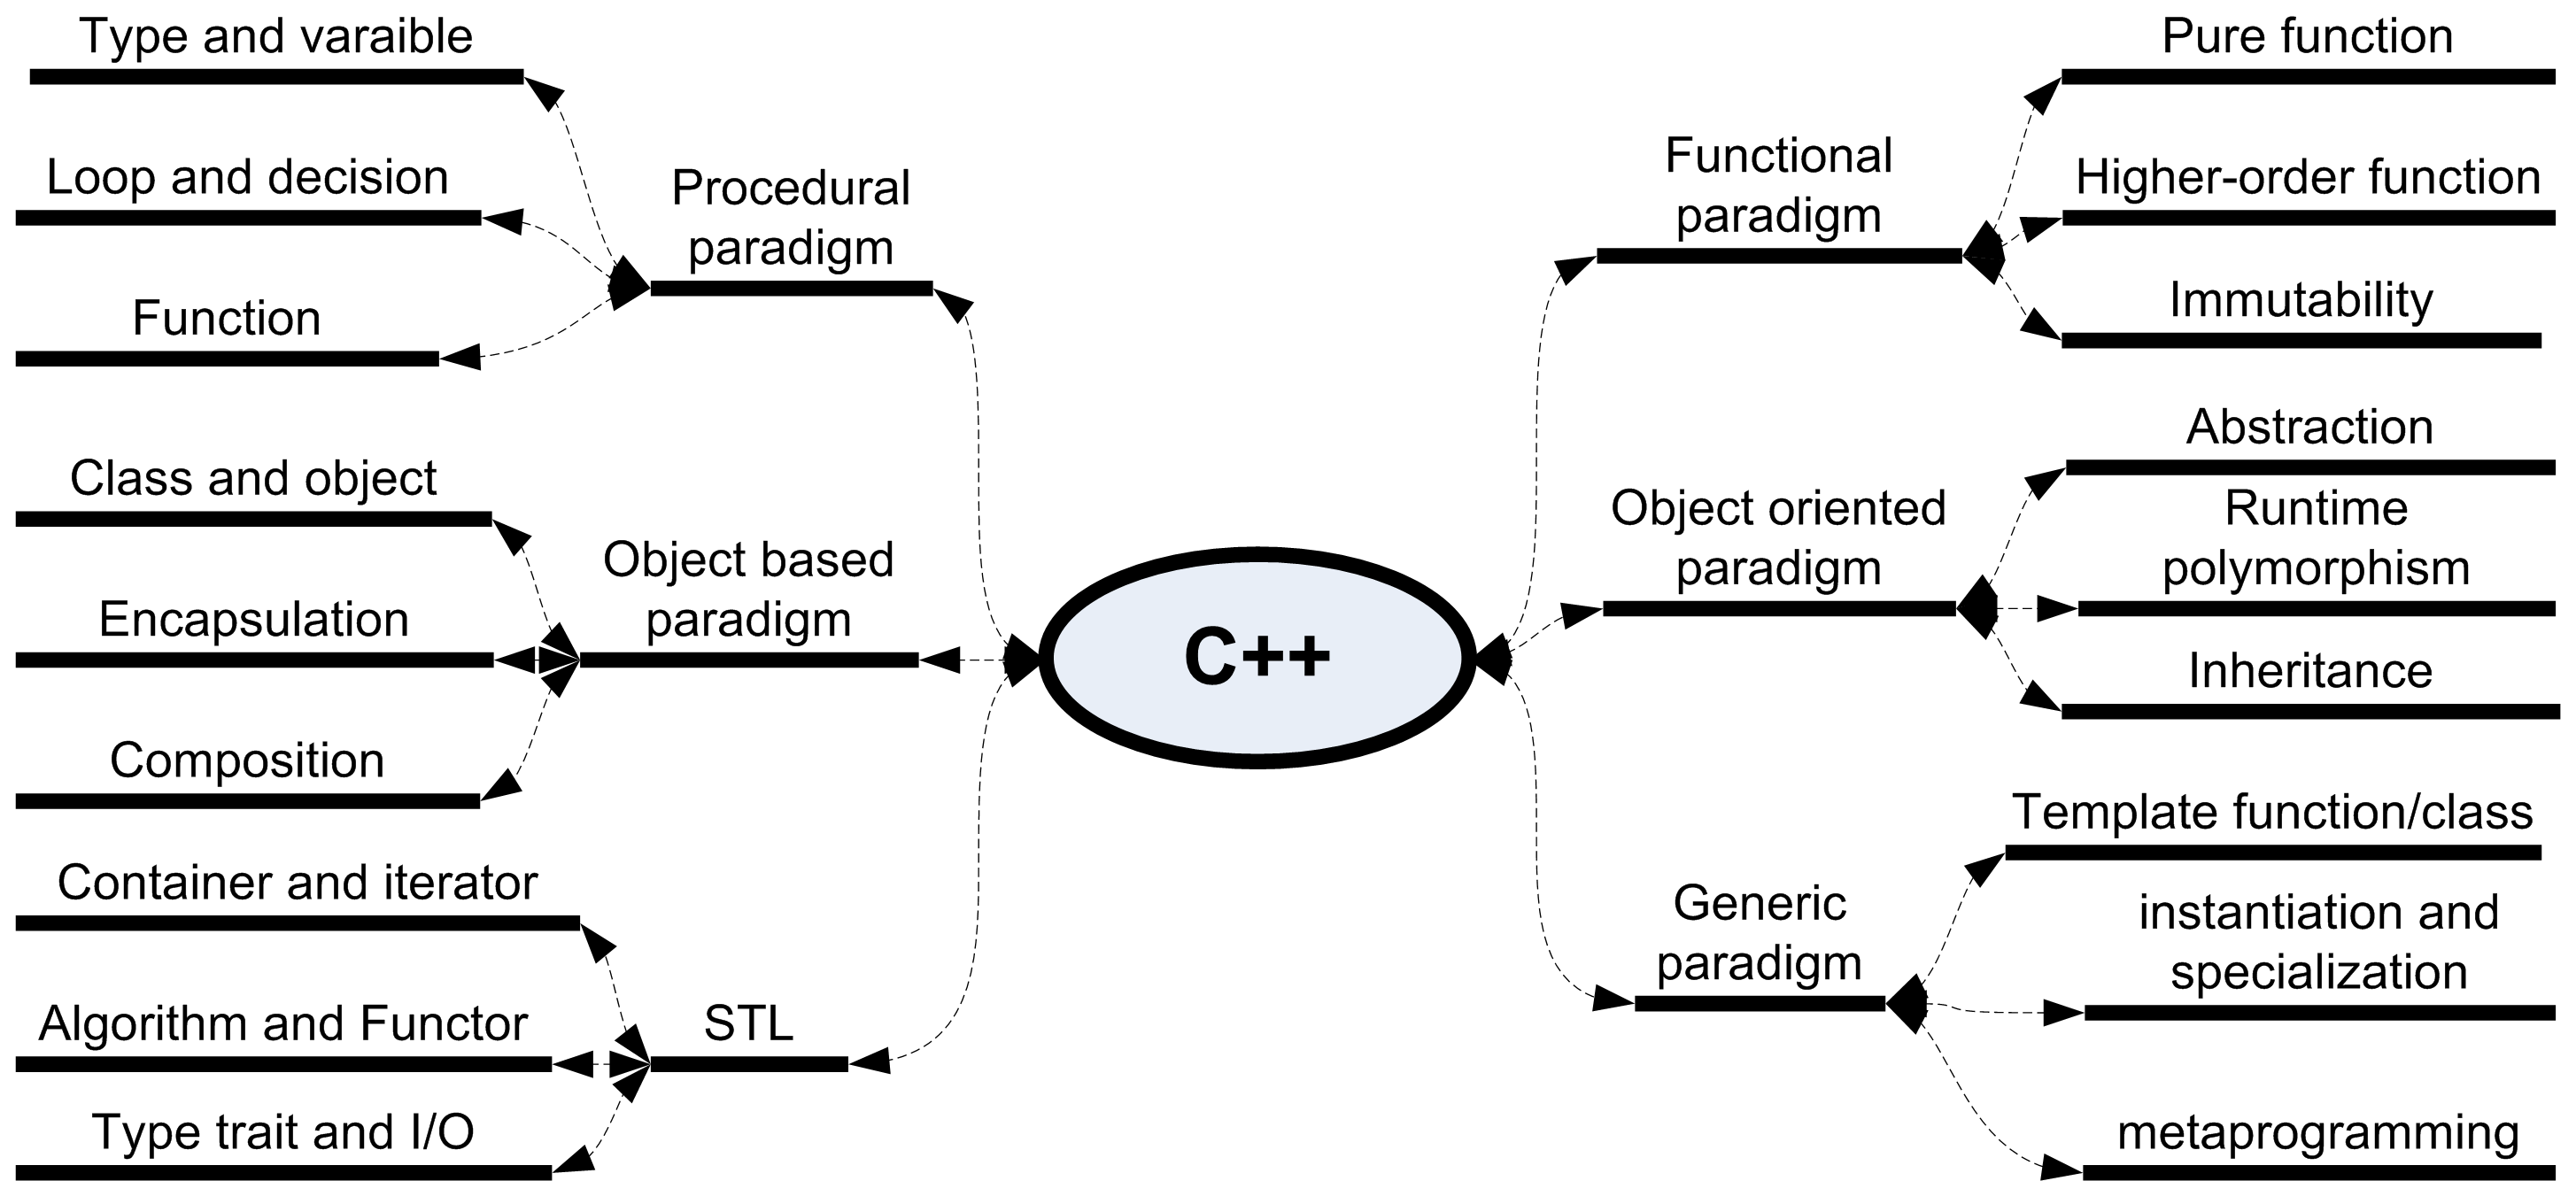
\includegraphics[width=0.85\linewidth]{pics/whole.png}
	%\caption{The main component of C++ language}



     \item C++ inherits basic data type, variable name, statement, expression, and operator, control flow, function, file, head file and library, array, pointer and structure from C language. C++ is superset of C, so any C programs can be compiled by C++.
    
    \item Duration and scope are two different conceptions in C++. there are three kinds of duration: \textbf{automatic, static and dynamic.} there are four kinds of scopes:
    \begin{enumerate}
        \item global.
        \item In C++, we can use namespace to add more scopes to divide global scope.
        \item file(translation unit).
        \item local, function local and class local. 
    \end{enumerate}
    
    \item Statement and expression are two important conceptions, you can see their definition in cppreference.com to see academic explanation.
    
    \item Statements are fragments of the C++ program that are executed in sequence. Only statement, which end with semicolon is executed. Most statements are expression statements. 
\begin{lstlisting}
x+y;  //is statement, but you throw away the result
int i; int i; int i;int i int i int ; int i;int ;float i; int i; int i; int i;int i int i int ; int i;int ;int i;
int i; int i; int i;int i int i int ; int i;int ;float i; int i; int i; int i;int i int i int ; int i;int ;int i;
\end{lstlisting}
\begin{description}
	\item[line 1:] There is more than one word.An expression is a sequence of \textbf{operators} and their \textbf{operands}, that specifies a computation. Expression evaluation may produce a resultAn expression is a sequence of \textbf{operators} and their \textbf{operands}, that specifies a computation. Expression evaluation may produce a result
	\item[line 3:] An expression is a sequence of \textbf{operators} and their \textbf{operands}, that specifies a computation. Expression evaluation may produce a resultAn expression is a sequence of \textbf{operators} and their \textbf{operands}, that specifies a computation. Expression evaluation may produce a result
\end{description}
\begin{enumerate}
	\item An expression is a sequence of \textbf{operators} and their \textbf{operands}, that specifies a computation. Expression evaluation may produce a resultAn expression is a sequence of \textbf{operators} and their \textbf{operands}, that specifies a computation. Expression evaluation may produce a result
	
	\item An expression is a sequence of \textbf{operators} and their \textbf{operands}, that specifies a computation. Expression evaluation may produce a resultAn expression is a sequence of \textbf{operators} and their \textbf{operands}, that specifies a computation. Expression evaluation may produce a result
\end{enumerate}
	\item An expression is a sequence of \textbf{operators} and their \textbf{operands}, that specifies a computation. Expression evaluation may produce a result

    \begin{enumerate}
    	\item Expression: Something which evaluates to a value. Example: \texttt{1+2/x}
    	\item Statement: A line of code which does something. Example: \texttt{GOTO 100;} and statements are all end with semi-comma.
    \end{enumerate}

    \item Function call is a expression, because it can yield a value.
    
    \item \textbf{All expressions yield a value, So expression is a value, statement is an action.}
    

    \item The designers of C realized that no harm was done if you were allowed to evaluate an expression and throw away the result. In C, every syntactic expression can be a made into a statement just by tacking a semicolon along the end:
    
\begin{lstlisting}[numbers=none]
x+y //is expression;
x+y; //is statement, but you throw away the result
j=i; is a statement.
fun(i) //is expression;
\end{lstlisting}
    
\end{itemize}

\subsection{basic definition}
\begin{itemize}
	
	\item gogo 
	
	
	\begin{tabular}{|c|c|c|}
		
		\textbf{type} & \textbf{read} & \textbf{write} \\
		
		primitive (char, int, float) & pass value & pointer or reference \\
		
		class, array, structure  & const pointer or reference &  pointer or reference  
	\end{tabular}
	\item gogo \newline
	

	
	\item gogo 
	
	\begin{tabular}{|p{0.3\textwidth}|p{0.3\textwidth}|p{0.3\textwidth}|}
		\tophline
		go go go go go go go let let let let let letgo go go go go go go let let let let let let &  go go go go go go go let let let let let letgo go go go go go go let let let let let let&
		go go go go go go go let let let let let letgo go go go go go go let let let let let let  
		\\ \tophline
		
		primitive (char, int, float) & pass value & pointer or reference \\ \tophline
		class, array, structure  & const pointer or reference &  pointer or reference \bottomhline
	\end{tabular}
	
	
	\item C++ is a Multi-paradigm language, there are five paradigms: 
	
	\begin{enumerate}
		\item Procedural programming. (traditional C programming)
		\item Object-base programming. (class and object)
		\item Object-orient programming. (inheritance)
		\item Generic programming. (template)
		\item functional programming
	\end{enumerate}
	
	
	%\centering
	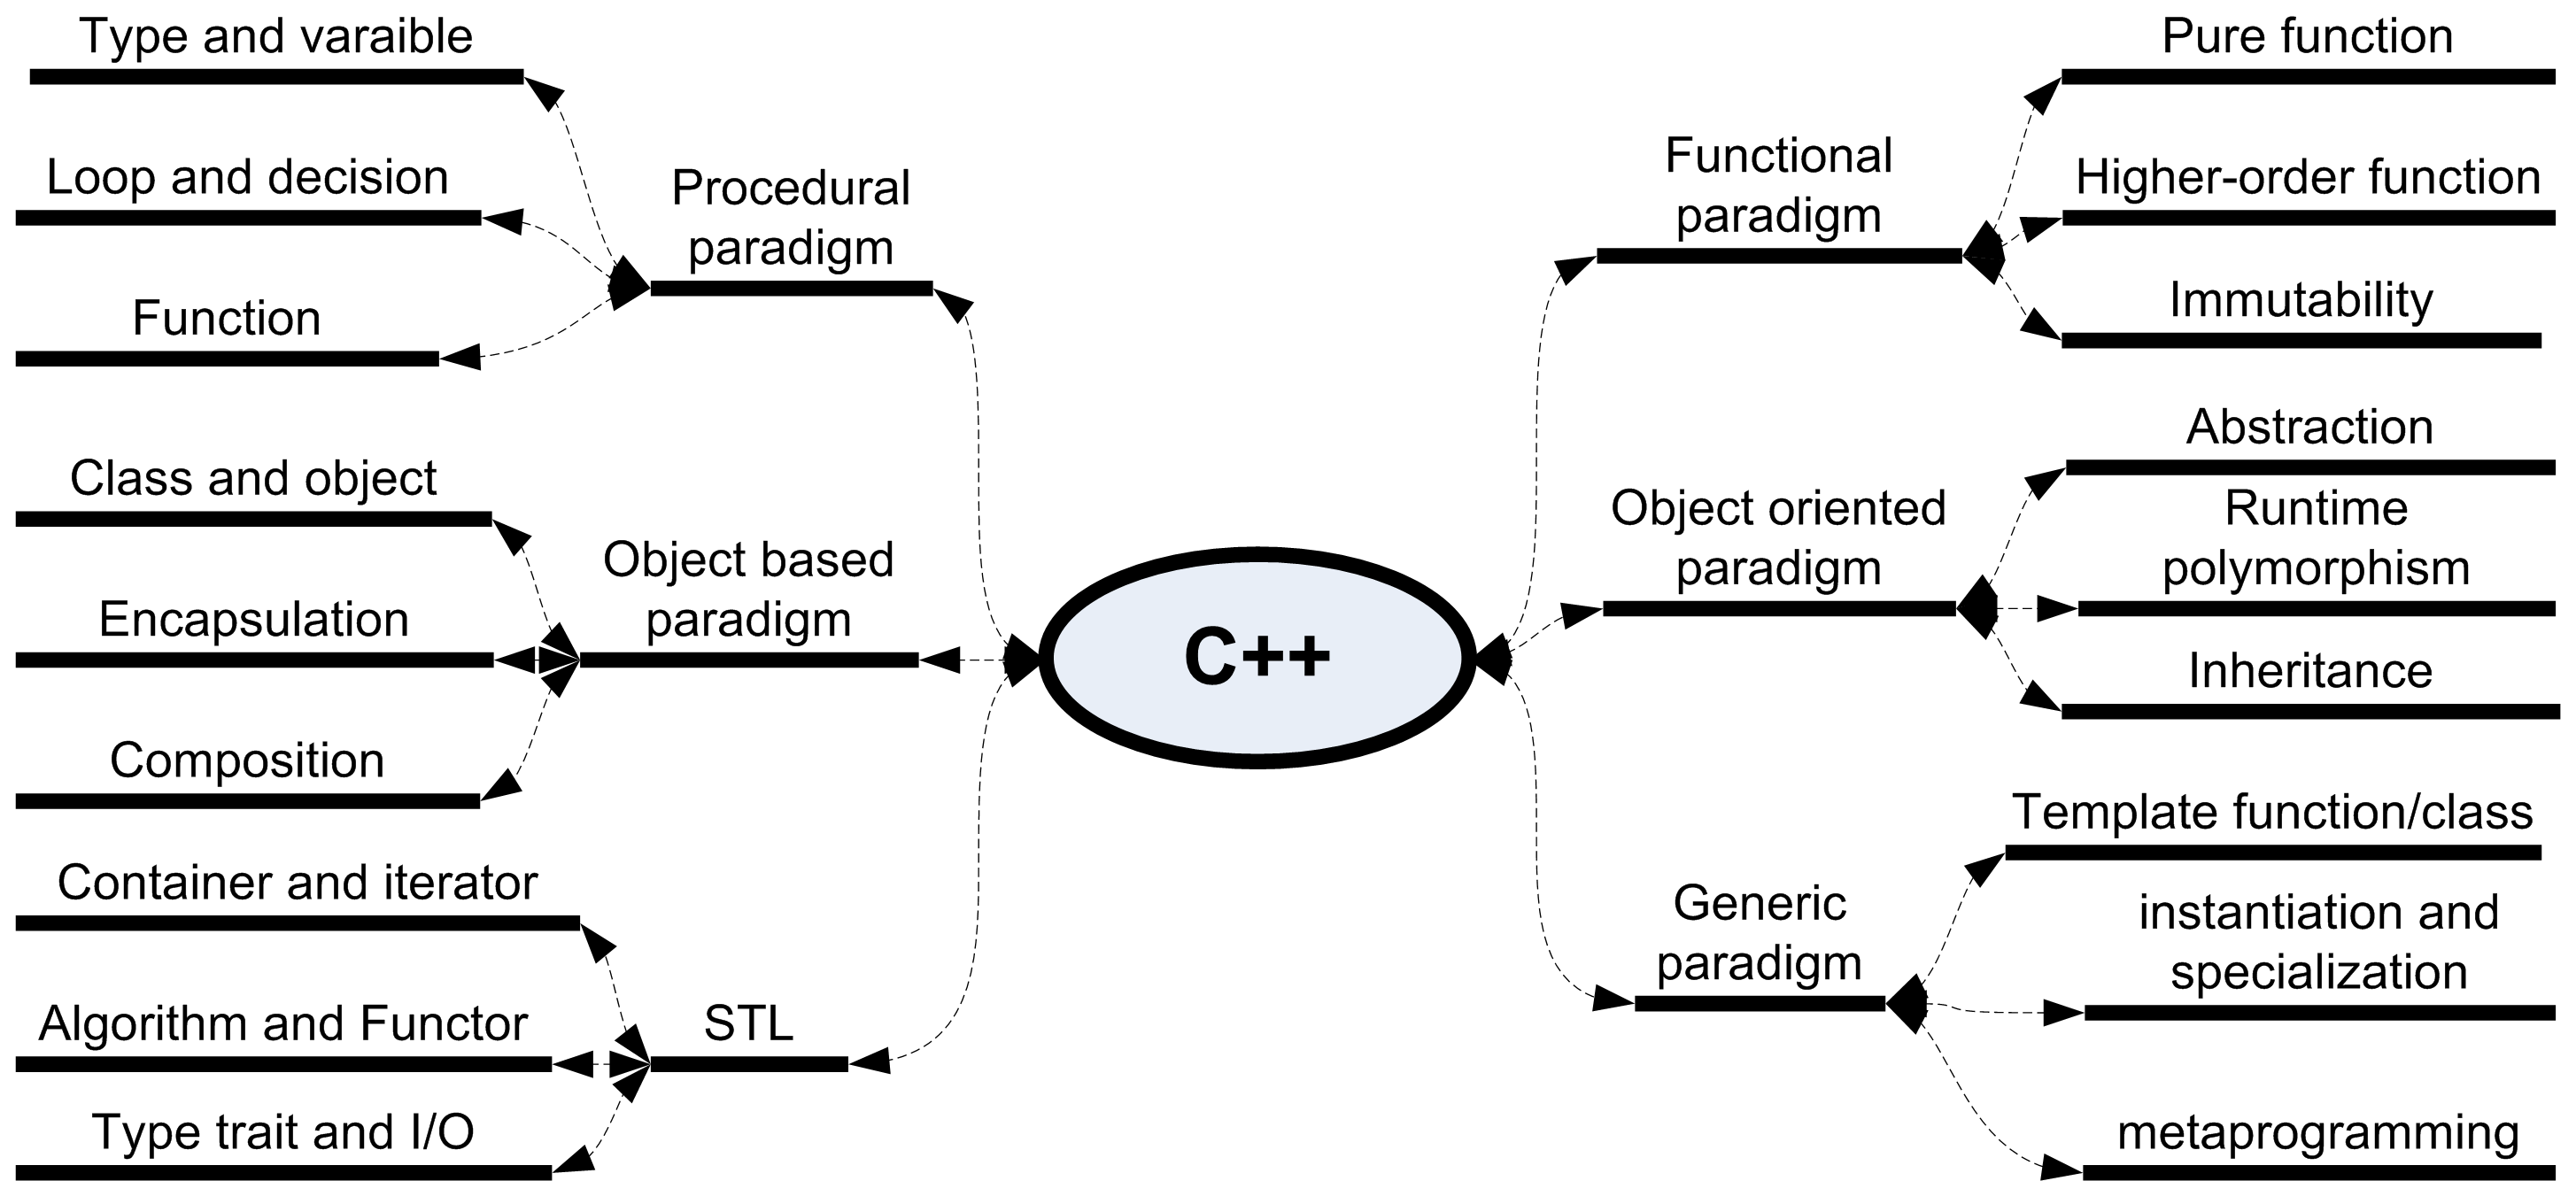
\includegraphics[width=0.85\linewidth]{pics/whole.png}
	%\caption{The main component of C++ language}
	
	
	
	\item C++ inherits basic data type, variable name, statement, expression, and operator, control flow, function, file, head file and library, array, pointer and structure from C language. C++ is superset of C, so any C programs can be compiled by C++.
	
	\item Duration and scope are two different conceptions in C++. there are three kinds of duration: \textbf{automatic, static and dynamic.} there are four kinds of scopes:
	\begin{enumerate}
		\item global.
		\item In C++, we can use namespace to add more scopes to divide global scope.
		\item file(translation unit).
		\item local, function local and class local. 
	\end{enumerate}
	
	\item Statement and expression are two important conceptions, you can see their definition in cppreference.com to see academic explanation.
	
	\item Statements are fragments of the C++ program that are executed in sequence. Only statement, which end with semicolon is executed. Most statements are expression statements. 
	\begin{lstlisting}
	int n = 1;               $\Hilight{3}$// declaration statement
	n = n + 1;               // expression statement
	std::cout << n << '\n'; // expression statement
	return 0;               // return statement stepnumber=1, 
	xleftmargin=1.2em, framexleftmargin=1.2em]
	int n = 1;               $\Hilight{3}$// declaration statement
	n = n + 1;               // expression statement
	std::cout << n << '\n'; // expression statement
	return 0;               // return statement
	stepnumber=1, xleftmargin=1.2em, framexleftmargin=1.2em]
	int n = 1;               $\Hilight{3}$// declaration statement
	n = n + 1;               // expression statement
	std::cout << n << '\n'; // expression statement
	return 0;               // return statement
	stepnumber=1, xleftmargin=1.2em, framexleftmargin=1.2em]
	int n = 1;               $\Hilight{3}$// declaration statement
	n = n + 1;               // expression statement
	std::cout << n << '\n'; // expression statement
	return 0;               // return statement
	\end{lstlisting}
	\begin{description}
		\item[line 1:] There is more than one word.An expression is a sequence of \textbf{operators} and their \textbf{operands}, that specifies a computation. Expression evaluation may produce a resultAn expression is a sequence of \textbf{operators} and their \textbf{operands}, that specifies a computation. Expression evaluation may produce a result
		\item[line 3:] An expression is a sequence of \textbf{operators} and their \textbf{operands}, that specifies a computation. Expression evaluation may produce a resultAn expression is a sequence of \textbf{operators} and their \textbf{operands}, that specifies a computation. Expression evaluation may produce a result
	\end{description}
	\begin{enumerate}
		\item An expression is a sequence of \textbf{operators} and their \textbf{operands}, that specifies a computation. Expression evaluation may produce a resultAn expression is a sequence of \textbf{operators} and their \textbf{operands}, that specifies a computation. Expression evaluation may produce a result
		
		\item An expression is a sequence of \textbf{operators} and their \textbf{operands}, that specifies a computation. Expression evaluation may produce a resultAn expression is a sequence of \textbf{operators} and their \textbf{operands}, that specifies a computation. Expression evaluation may produce a result
	\end{enumerate}
	\item An expression is a sequence of \textbf{operators} and their \textbf{operands}, that specifies a computation. Expression evaluation may produce a result
	
	\begin{enumerate}
		\item Expression: Something which evaluates to a value. Example: \texttt{1+2/x}
		\item Statement: A line of code which does something. Example: \texttt{GOTO 100;} and statements are all end with semi-comma.
	\end{enumerate}
	
	\item Function call is a expression, because it can yield a value.
	
	\item \textbf{All expressions yield a value, So expression is a value, statement is an action.}
	
	
	\item The designers of C realized that no harm was done if you were allowed to evaluate an expression and throw away the result. In C, every syntactic expression can be a made into a statement just by tacking a semicolon along the end:
	
	\begin{lstlisting}[numbers=none]
	x+y //is expression;
	x+y; //is statement, but you throw away the result
	j=i; is a statement.
	fun(i) //is expression;
	\end{lstlisting}
	
\end{itemize}

\subsection{basic definition}
\begin{itemize}
	
	\item gogo 
	
	
	\begin{tabular}{|c|c|c|}
		
		\textbf{type} & \textbf{read} & \textbf{write} \\
		
		primitive (char, int, float) & pass value & pointer or reference \\
		
		class, array, structure  & const pointer or reference &  pointer or reference  
	\end{tabular}
	\item gogo \newline
	
	
	
	\item gogo 
	
	\begin{tabular}{|p{0.3\textwidth}|p{0.3\textwidth}|p{0.3\textwidth}|}
		\tophline
		go go go go go go go let let let let let letgo go go go go go go let let let let let let &  go go go go go go go let let let let let letgo go go go go go go let let let let let let&
		go go go go go go go let let let let let letgo go go go go go go let let let let let let  
		\\ \tophline
		
		primitive (char, int, float) & pass value & pointer or reference \\ \tophline
		class, array, structure  & const pointer or reference &  pointer or reference \bottomhline
	\end{tabular}
	
	
	\item C++ is a Multi-paradigm language, there are five paradigms: 
	
	\begin{enumerate}
		\item Procedural programming. (traditional C programming)
		\item Object-base programming. (class and object)
		\item Object-orient programming. (inheritance)
		\item Generic programming. (template)
		\item functional programming
	\end{enumerate}
	
	
	%\centering
	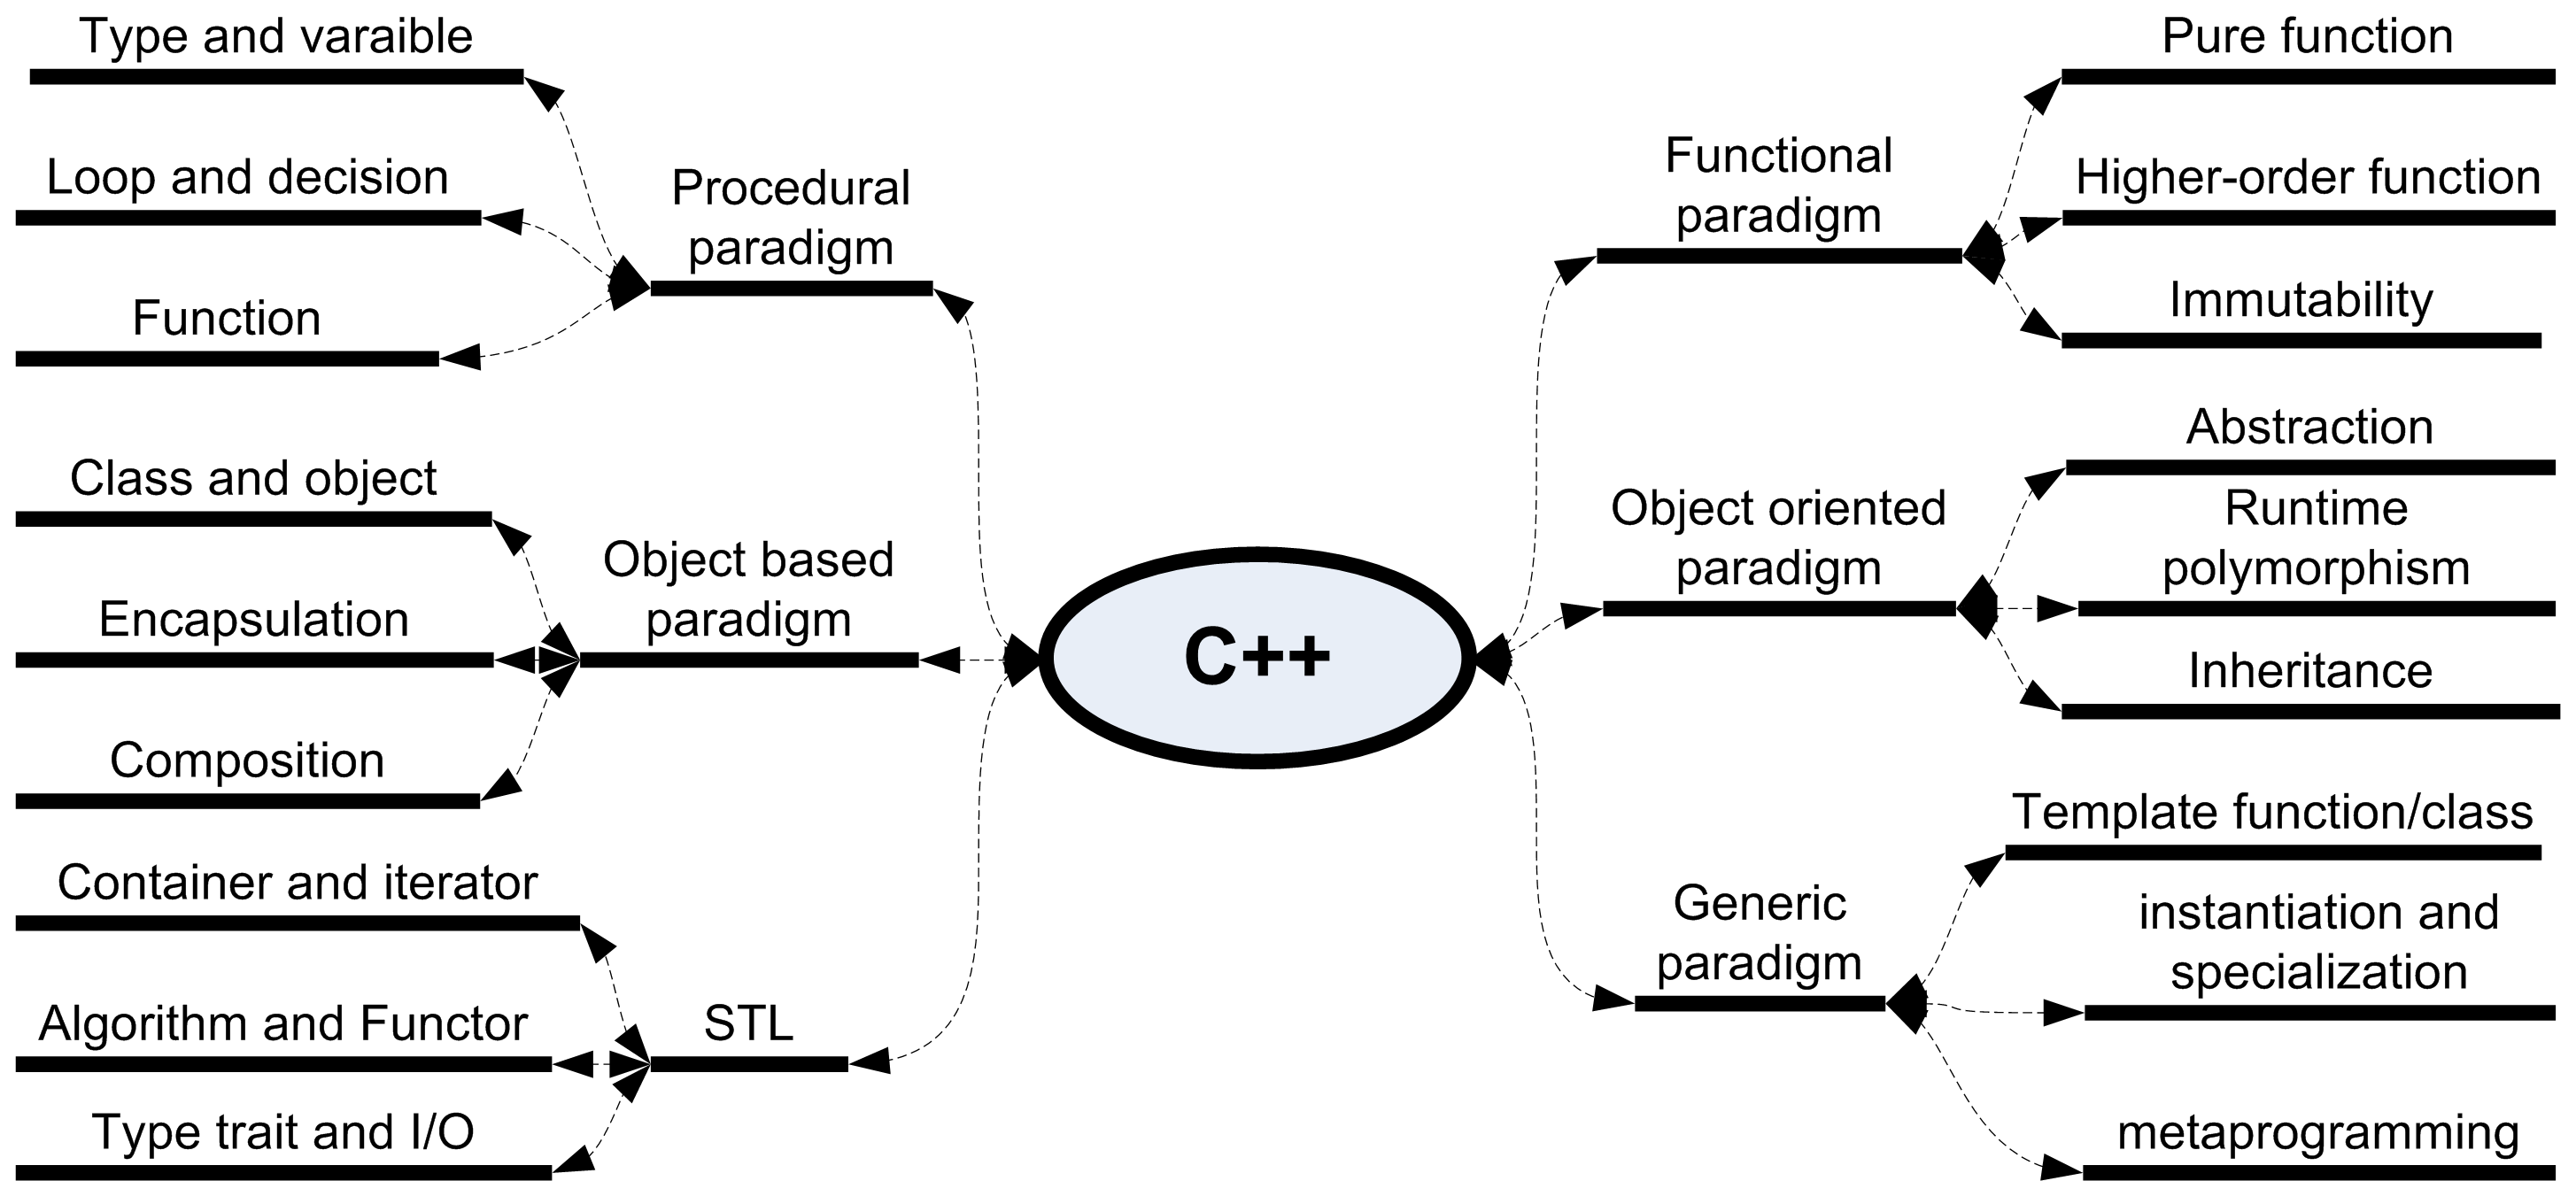
\includegraphics[width=0.85\linewidth]{pics/whole.png}
	%\caption{The main component of C++ language}
	
	
	
	\item C++ inherits basic data type, variable name, statement, expression, and operator, control flow, function, file, head file and library, array, pointer and structure from C language. C++ is superset of C, so any C programs can be compiled by C++.
	
	\item Duration and scope are two different conceptions in C++. there are three kinds of duration: \textbf{automatic, static and dynamic.} there are four kinds of scopes:
	\begin{enumerate}
		\item global.
		\item In C++, we can use namespace to add more scopes to divide global scope.
		\item file(translation unit).
		\item local, function local and class local. 
	\end{enumerate}
	
	\item Statement and expression are two important conceptions, you can see their definition in cppreference.com to see academic explanation.
	
	\item Statements are fragments of the C++ program that are executed in sequence. Only statement, which end with semicolon is executed. Most statements are expression statements. 
	\begin{lstlisting}
	int n = 1;               $\Hilight{3}$// declaration statement
	n = n + 1;               // expression statement
	std::cout << n << '\n'; // expression statement
	return 0;               // return statement stepnumber=1, 
	xleftmargin=1.2em, framexleftmargin=1.2em]
	int n = 1;               $\Hilight{3}$// declaration statement
	n = n + 1;               // expression statement
	std::cout << n << '\n'; // expression statement
	return 0;               // return statement
	stepnumber=1, xleftmargin=1.2em, framexleftmargin=1.2em]
	int n = 1;               $\Hilight{3}$// declaration statement
	n = n + 1;               // expression statement
	std::cout << n << '\n'; // expression statement
	return 0;               // return statement
	stepnumber=1, xleftmargin=1.2em, framexleftmargin=1.2em]
	int n = 1;               $\Hilight{3}$// declaration statement
	n = n + 1;               // expression statement
	std::cout << n << '\n'; // expression statement
	return 0;               // return statement
	\end{lstlisting}
	\begin{description}
		\item[line 1:] There is more than one word.An expression is a sequence of \textbf{operators} and their \textbf{operands}, that specifies a computation. Expression evaluation may produce a resultAn expression is a sequence of \textbf{operators} and their \textbf{operands}, that specifies a computation. Expression evaluation may produce a result
		\item[line 3:] An expression is a sequence of \textbf{operators} and their \textbf{operands}, that specifies a computation. Expression evaluation may produce a resultAn expression is a sequence of \textbf{operators} and their \textbf{operands}, that specifies a computation. Expression evaluation may produce a result
	\end{description}
	\begin{enumerate}
		\item An expression is a sequence of \textbf{operators} and their \textbf{operands}, that specifies a computation. Expression evaluation may produce a resultAn expression is a sequence of \textbf{operators} and their \textbf{operands}, that specifies a computation. Expression evaluation may produce a result
		
		\item An expression is a sequence of \textbf{operators} and their \textbf{operands}, that specifies a computation. Expression evaluation may produce a resultAn expression is a sequence of \textbf{operators} and their \textbf{operands}, that specifies a computation. Expression evaluation may produce a result
	\end{enumerate}
	\item An expression is a sequence of \textbf{operators} and their \textbf{operands}, that specifies a computation. Expression evaluation may produce a result
	
	\begin{enumerate}
		\item Expression: Something which evaluates to a value. Example: \texttt{1+2/x}
		\item Statement: A line of code which does something. Example: \texttt{GOTO 100;} and statements are all end with semi-comma.
	\end{enumerate}
	
	\item Function call is a expression, because it can yield a value.
	
	\item \textbf{All expressions yield a value, So expression is a value, statement is an action.}
	
	
	\item The designers of C realized that no harm was done if you were allowed to evaluate an expression and throw away the result. In C, every syntactic expression can be a made into a statement just by tacking a semicolon along the end:
	
	\begin{lstlisting}[numbers=none]
	x+y //is expression;
	x+y; //is statement, but you throw away the result
	j=i; is a statement.
	fun(i) //is expression;
	\end{lstlisting}
	
\end{itemize}


\subsection{basic definition}
\begin{itemize}
	
	\item gogo 
	
	
	\begin{tabular}{|c|c|c|}
		
		\textbf{type} & \textbf{read} & \textbf{write} \\
		
		primitive (char, int, float) & pass value & pointer or reference \\
		
		class, array, structure  & const pointer or reference &  pointer or reference  
	\end{tabular}
	\item gogo \newline
	
	
	
	\item gogo 
	
	\begin{tabular}{|p{0.3\textwidth}|p{0.3\textwidth}|p{0.3\textwidth}|}
		\tophline
		go go go go go go go let let let let let letgo go go go go go go let let let let let let &  go go go go go go go let let let let let letgo go go go go go go let let let let let let&
		go go go go go go go let let let let let letgo go go go go go go let let let let let let  
		\\ \tophline
		
		primitive (char, int, float) & pass value & pointer or reference \\ \tophline
		class, array, structure  & const pointer or reference &  pointer or reference \bottomhline
	\end{tabular}
	
	
	\item C++ is a Multi-paradigm language, there are five paradigms: 
	
	\begin{enumerate}
		\item Procedural programming. (traditional C programming)
		\item Object-base programming. (class and object)
		\item Object-orient programming. (inheritance)
		\item Generic programming. (template)
		\item functional programming
	\end{enumerate}
	
	
	%\centering
	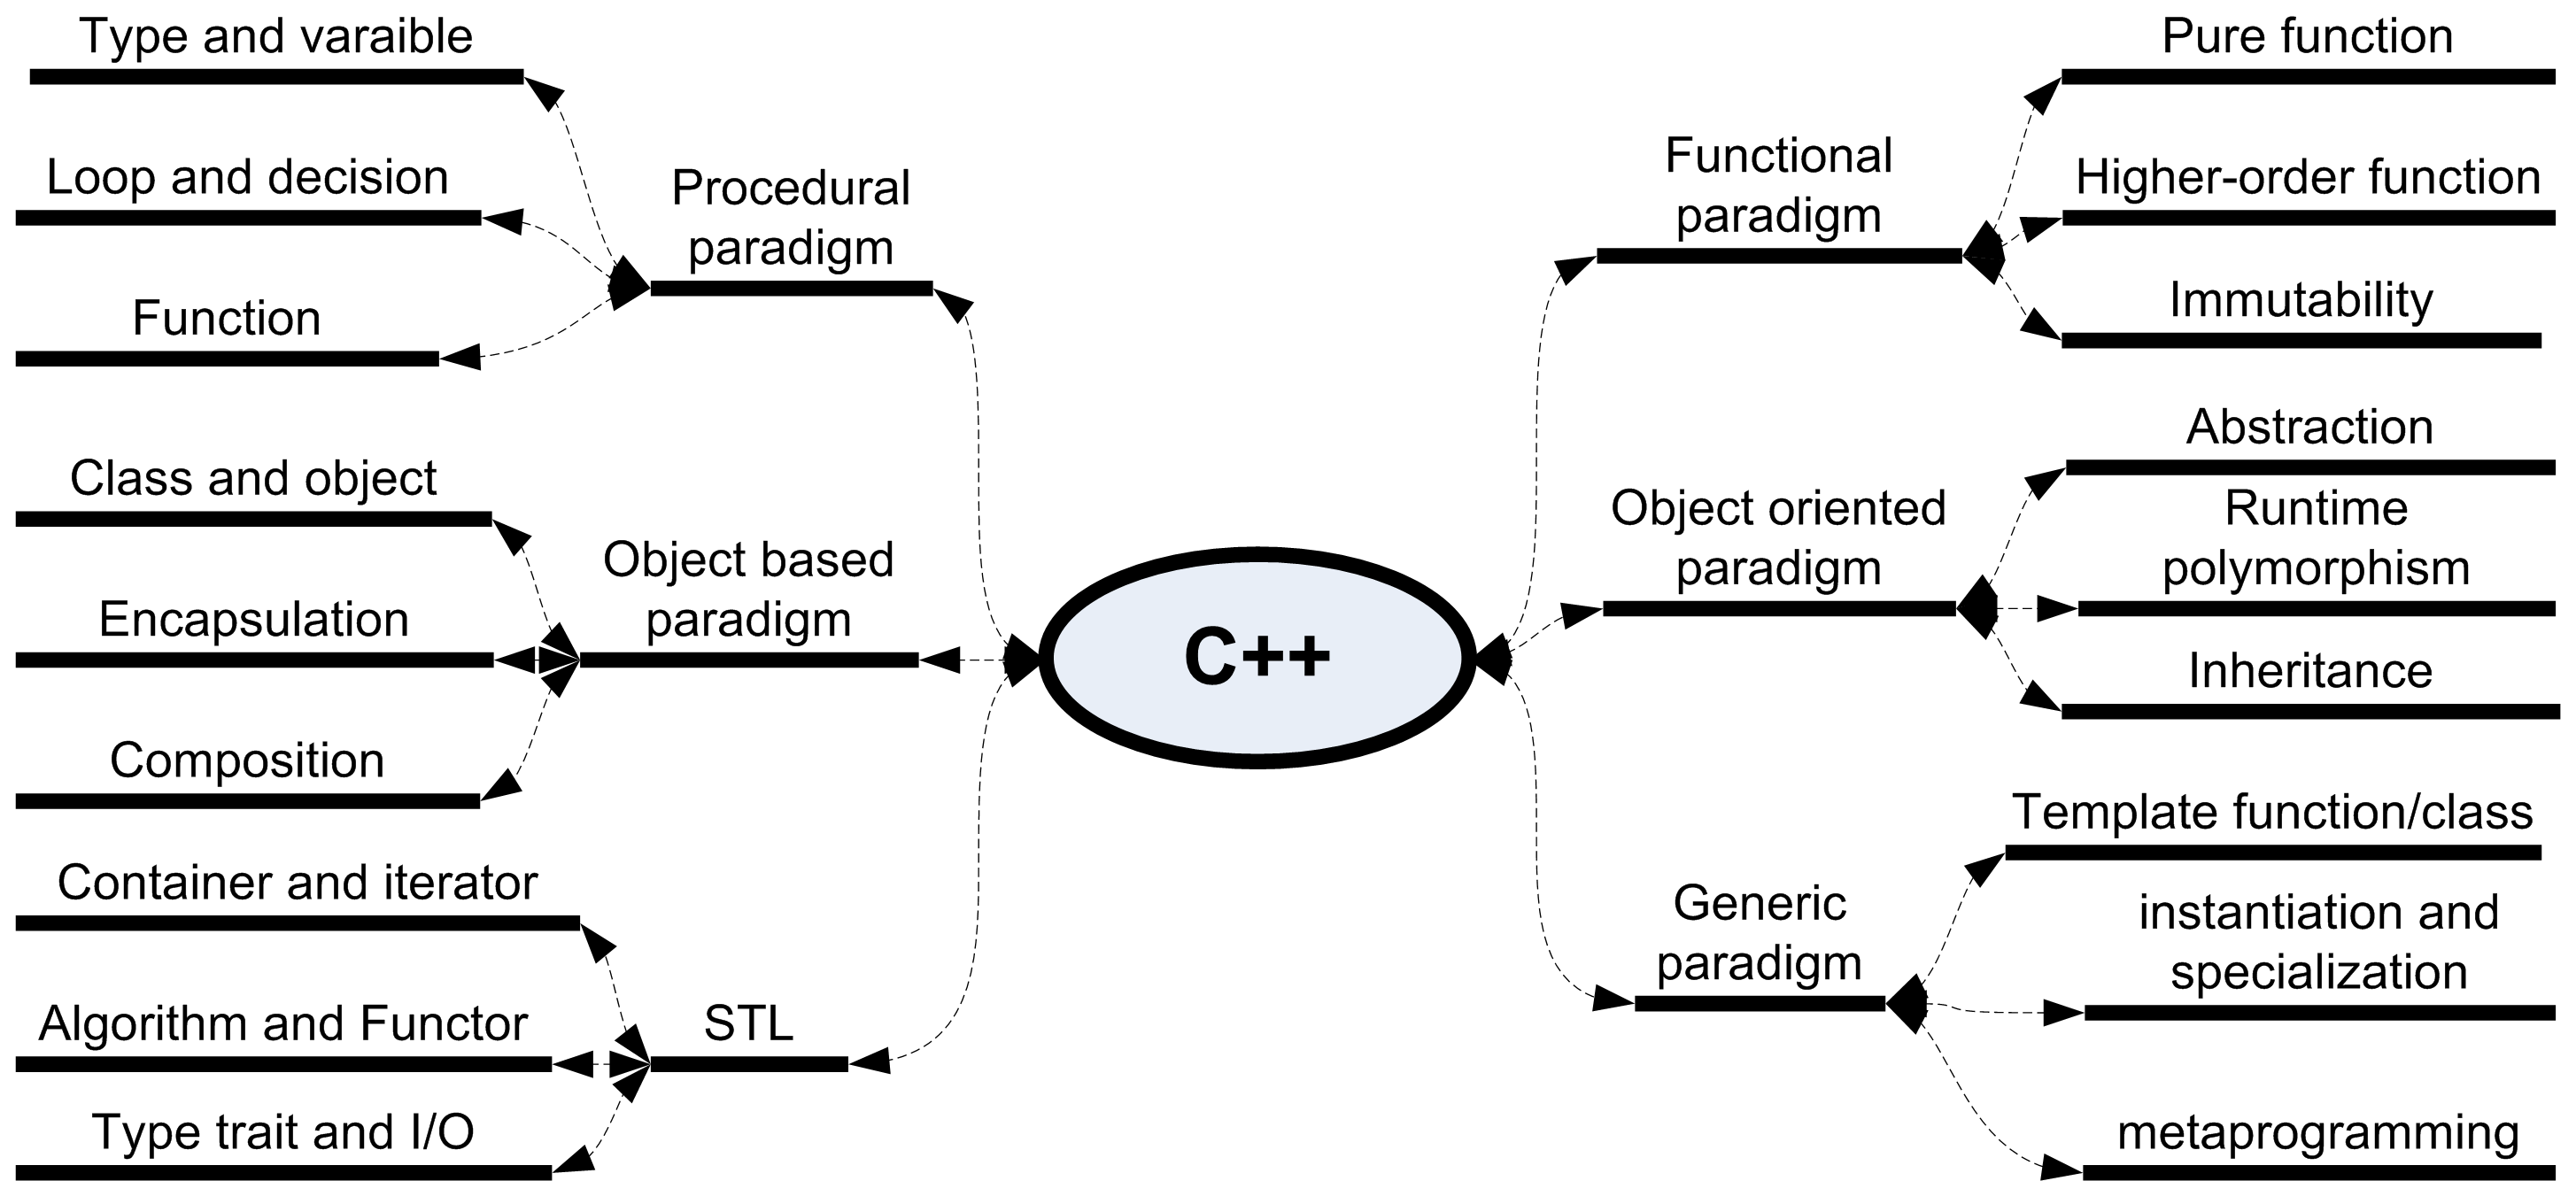
\includegraphics[width=0.85\linewidth]{pics/whole.png}
	%\caption{The main component of C++ language}
	
	
	
	\item C++ inherits basic data type, variable name, statement, expression, and operator, control flow, function, file, head file and library, array, pointer and structure from C language. C++ is superset of C, so any C programs can be compiled by C++.
	
	\item Duration and scope are two different conceptions in C++. there are three kinds of duration: \textbf{automatic, static and dynamic.} there are four kinds of scopes:
	\begin{enumerate}
		\item global.
		\item In C++, we can use namespace to add more scopes to divide global scope.
		\item file(translation unit).
		\item local, function local and class local. 
	\end{enumerate}
	
	\item Statement and expression are two important conceptions, you can see their definition in cppreference.com to see academic explanation.
	
	\item Statements are fragments of the C++ program that are executed in sequence. Only statement, which end with semicolon is executed. Most statements are expression statements. 
	\begin{lstlisting}
	int n = 1;               $\Hilight{3}$// declaration statement
	n = n + 1;               // expression statement
	std::cout << n << '\n'; // expression statement
	return 0;               // return statement stepnumber=1, 
	xleftmargin=1.2em, framexleftmargin=1.2em]
	int n = 1;               $\Hilight{3}$// declaration statement
	n = n + 1;               // expression statement
	std::cout << n << '\n'; // expression statement
	return 0;               // return statement
	stepnumber=1, xleftmargin=1.2em, framexleftmargin=1.2em]
	int n = 1;               $\Hilight{3}$// declaration statement
	n = n + 1;               // expression statement
	std::cout << n << '\n'; // expression statement
	return 0;               // return statement
	stepnumber=1, xleftmargin=1.2em, framexleftmargin=1.2em]
	int n = 1;               $\Hilight{3}$// declaration statement
	n = n + 1;               // expression statement
	std::cout << n << '\n'; // expression statement
	return 0;               // return statement
	\end{lstlisting}
	\begin{description}
		\item[line 1:] There is more than one word.An expression is a sequence of \textbf{operators} and their \textbf{operands}, that specifies a computation. Expression evaluation may produce a resultAn expression is a sequence of \textbf{operators} and their \textbf{operands}, that specifies a computation. Expression evaluation may produce a result
		\item[line 3:] An expression is a sequence of \textbf{operators} and their \textbf{operands}, that specifies a computation. Expression evaluation may produce a resultAn expression is a sequence of \textbf{operators} and their \textbf{operands}, that specifies a computation. Expression evaluation may produce a result
	\end{description}
	\begin{enumerate}
		\item An expression is a sequence of \textbf{operators} and their \textbf{operands}, that specifies a computation. Expression evaluation may produce a resultAn expression is a sequence of \textbf{operators} and their \textbf{operands}, that specifies a computation. Expression evaluation may produce a result
		
		\item An expression is a sequence of \textbf{operators} and their \textbf{operands}, that specifies a computation. Expression evaluation may produce a resultAn expression is a sequence of \textbf{operators} and their \textbf{operands}, that specifies a computation. Expression evaluation may produce a result
	\end{enumerate}
	\item An expression is a sequence of \textbf{operators} and their \textbf{operands}, that specifies a computation. Expression evaluation may produce a result
	
	\begin{enumerate}
		\item Expression: Something which evaluates to a value. Example: \texttt{1+2/x}
		\item Statement: A line of code which does something. Example: \texttt{GOTO 100;} and statements are all end with semi-comma.
	\end{enumerate}
	
	\item Function call is a expression, because it can yield a value.
	
	\item \textbf{All expressions yield a value, So expression is a value, statement is an action.}
	
	
	\item The designers of C realized that no harm was done if you were allowed to evaluate an expression and throw away the result. In C, every syntactic expression can be a made into a statement just by tacking a semicolon along the end:
	
	\begin{lstlisting}[numbers=none]
	x+y //is expression;
	x+y; //is statement, but you throw away the result
	j=i; is a statement.
	fun(i) //is expression;
	\end{lstlisting}
	
\end{itemize}


\subsection{basic definition}
\begin{itemize}
	
	\item gogo 
	
	
	\begin{tabular}{|c|c|c|}
		
		\textbf{type} & \textbf{read} & \textbf{write} \\
		
		primitive (char, int, float) & pass value & pointer or reference \\
		
		class, array, structure  & const pointer or reference &  pointer or reference  
	\end{tabular}
	\item gogo \newline
	
	
	
	\item gogo 
	
	\begin{tabular}{|p{0.3\textwidth}|p{0.3\textwidth}|p{0.3\textwidth}|}
		\tophline
		go go go go go go go let let let let let letgo go go go go go go let let let let let let &  go go go go go go go let let let let let letgo go go go go go go let let let let let let&
		go go go go go go go let let let let let letgo go go go go go go let let let let let let  
		\\ \tophline
		
		primitive (char, int, float) & pass value & pointer or reference \\ \tophline
		class, array, structure  & const pointer or reference &  pointer or reference \bottomhline
	\end{tabular}
	
	
	\item C++ is a Multi-paradigm language, there are five paradigms: 
	
	\begin{enumerate}
		\item Procedural programming. (traditional C programming)
		\item Object-base programming. (class and object)
		\item Object-orient programming. (inheritance)
		\item Generic programming. (template)
		\item functional programming
	\end{enumerate}
	
	
	%\centering
	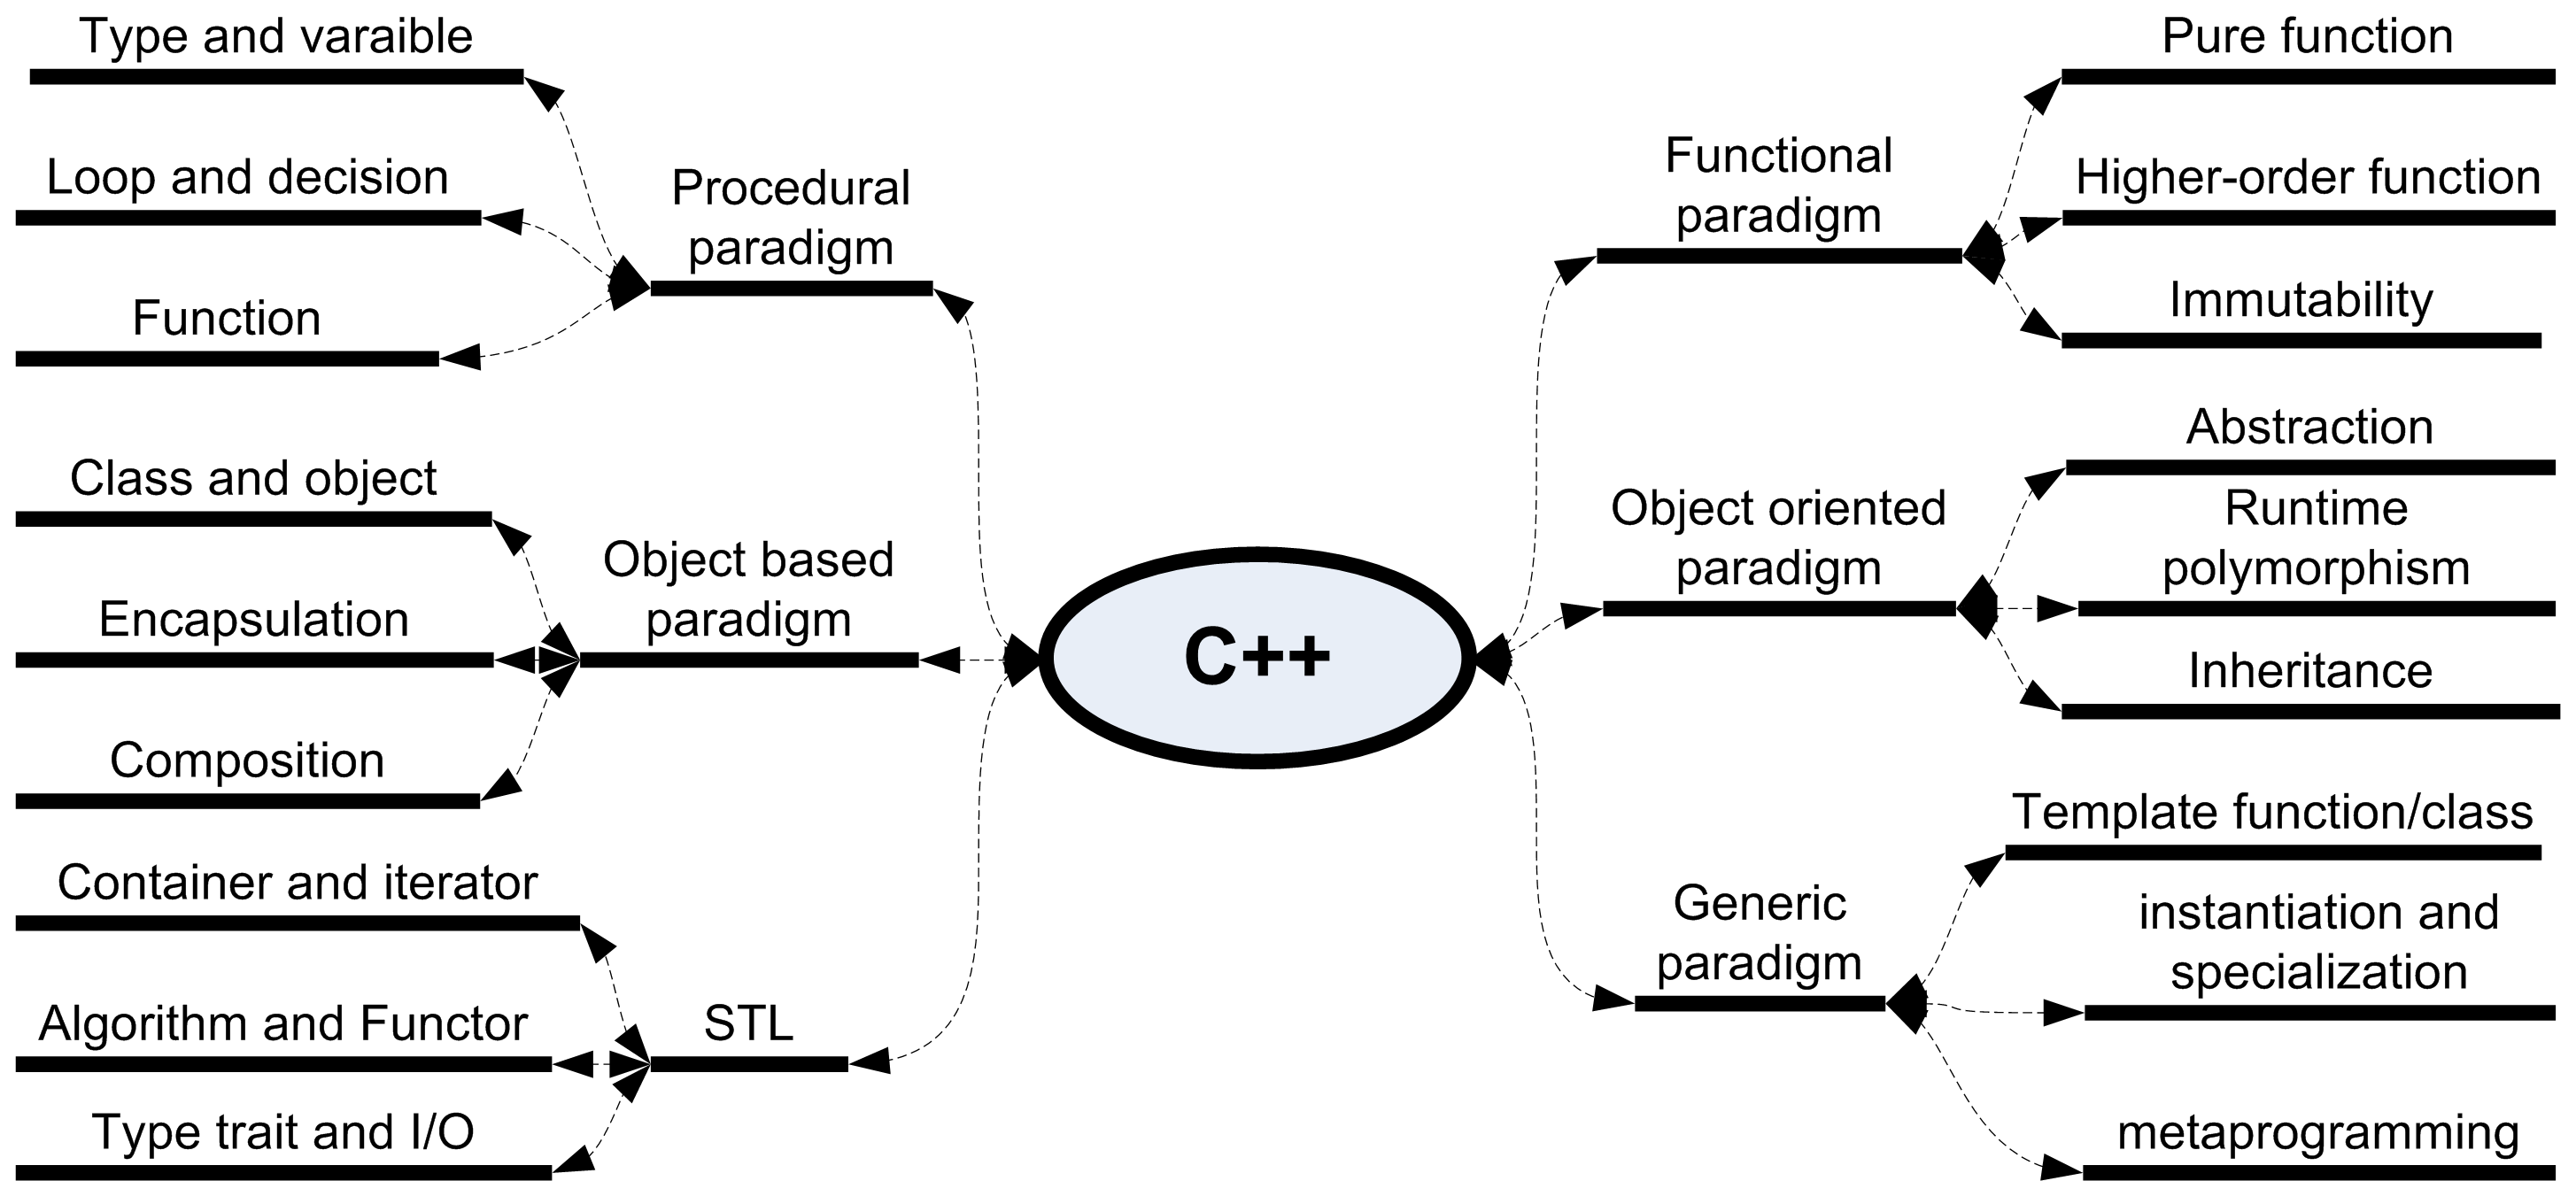
\includegraphics[width=0.85\linewidth]{pics/whole.png}
	%\caption{The main component of C++ language}
	
	
	
	\item C++ inherits basic data type, variable name, statement, expression, and operator, control flow, function, file, head file and library, array, pointer and structure from C language. C++ is superset of C, so any C programs can be compiled by C++.
	
	\item Duration and scope are two different conceptions in C++. there are three kinds of duration: \textbf{automatic, static and dynamic.} there are four kinds of scopes:
	\begin{enumerate}
		\item global.
		\item In C++, we can use namespace to add more scopes to divide global scope.
		\item file(translation unit).
		\item local, function local and class local. 
	\end{enumerate}
	
	\item Statement and expression are two important conceptions, you can see their definition in cppreference.com to see academic explanation.
	
	\item Statements are fragments of the C++ program that are executed in sequence. Only statement, which end with semicolon is executed. Most statements are expression statements. 
	\begin{lstlisting}
	int n = 1;               $\Hilight{3}$// declaration statement
	n = n + 1;               // expression statement
	std::cout << n << '\n'; // expression statement
	return 0;               // return statement stepnumber=1, 
	xleftmargin=1.2em, framexleftmargin=1.2em]
	int n = 1;               $\Hilight{3}$// declaration statement
	n = n + 1;               // expression statement
	std::cout << n << '\n'; // expression statement
	return 0;               // return statement
	stepnumber=1, xleftmargin=1.2em, framexleftmargin=1.2em]
	int n = 1;               $\Hilight{3}$// declaration statement
	n = n + 1;               // expression statement
	std::cout << n << '\n'; // expression statement
	return 0;               // return statement
	stepnumber=1, xleftmargin=1.2em, framexleftmargin=1.2em]
	int n = 1;               $\Hilight{3}$// declaration statement
	n = n + 1;               // expression statement
	std::cout << n << '\n'; // expression statement
	return 0;               // return statement
	\end{lstlisting}
	\begin{description}
		\item[line 1:] There is more than one word.An expression is a sequence of \textbf{operators} and their \textbf{operands}, that specifies a computation. Expression evaluation may produce a resultAn expression is a sequence of \textbf{operators} and their \textbf{operands}, that specifies a computation. Expression evaluation may produce a result
		\item[line 3:] An expression is a sequence of \textbf{operators} and their \textbf{operands}, that specifies a computation. Expression evaluation may produce a resultAn expression is a sequence of \textbf{operators} and their \textbf{operands}, that specifies a computation. Expression evaluation may produce a result
	\end{description}
	\begin{enumerate}
		\item An expression is a sequence of \textbf{operators} and their \textbf{operands}, that specifies a computation. Expression evaluation may produce a resultAn expression is a sequence of \textbf{operators} and their \textbf{operands}, that specifies a computation. Expression evaluation may produce a result
		
		\item An expression is a sequence of \textbf{operators} and their \textbf{operands}, that specifies a computation. Expression evaluation may produce a resultAn expression is a sequence of \textbf{operators} and their \textbf{operands}, that specifies a computation. Expression evaluation may produce a result
	\end{enumerate}
	\item An expression is a sequence of \textbf{operators} and their \textbf{operands}, that specifies a computation. Expression evaluation may produce a result
	
	\begin{enumerate}
		\item Expression: Something which evaluates to a value. Example: \texttt{1+2/x}
		\item Statement: A line of code which does something. Example: \texttt{GOTO 100;} and statements are all end with semi-comma.
	\end{enumerate}
	
	\item Function call is a expression, because it can yield a value.
	
	\item \textbf{All expressions yield a value, So expression is a value, statement is an action.}
	
	
	\item The designers of C realized that no harm was done if you were allowed to evaluate an expression and throw away the result. In C, every syntactic expression can be a made into a statement just by tacking a semicolon along the end:
	
	\begin{lstlisting}[numbers=none]
	x+y //is expression;
	x+y; //is statement, but you throw away the result
	j=i; is a statement.
	fun(i) //is expression;
	\end{lstlisting}
	
\end{itemize}


\subsection{basic definition}
\begin{itemize}
	
	\item gogo 
	
	
	\begin{tabular}{|c|c|c|}
		
		\textbf{type} & \textbf{read} & \textbf{write} \\
		
		primitive (char, int, float) & pass value & pointer or reference \\
		
		class, array, structure  & const pointer or reference &  pointer or reference  
	\end{tabular}
	\item gogo \newline
	
	
	
	\item gogo 
	
	\begin{tabular}{|p{0.3\textwidth}|p{0.3\textwidth}|p{0.3\textwidth}|}
		\tophline
		go go go go go go go let let let let let letgo go go go go go go let let let let let let &  go go go go go go go let let let let let letgo go go go go go go let let let let let let&
		go go go go go go go let let let let let letgo go go go go go go let let let let let let  
		\\ \tophline
		
		primitive (char, int, float) & pass value & pointer or reference \\ \tophline
		class, array, structure  & const pointer or reference &  pointer or reference \bottomhline
	\end{tabular}
	
	
	\item C++ is a Multi-paradigm language, there are five paradigms: 
	
	\begin{enumerate}
		\item Procedural programming. (traditional C programming)
		\item Object-base programming. (class and object)
		\item Object-orient programming. (inheritance)
		\item Generic programming. (template)
		\item functional programming
	\end{enumerate}
	
	
	%\centering
	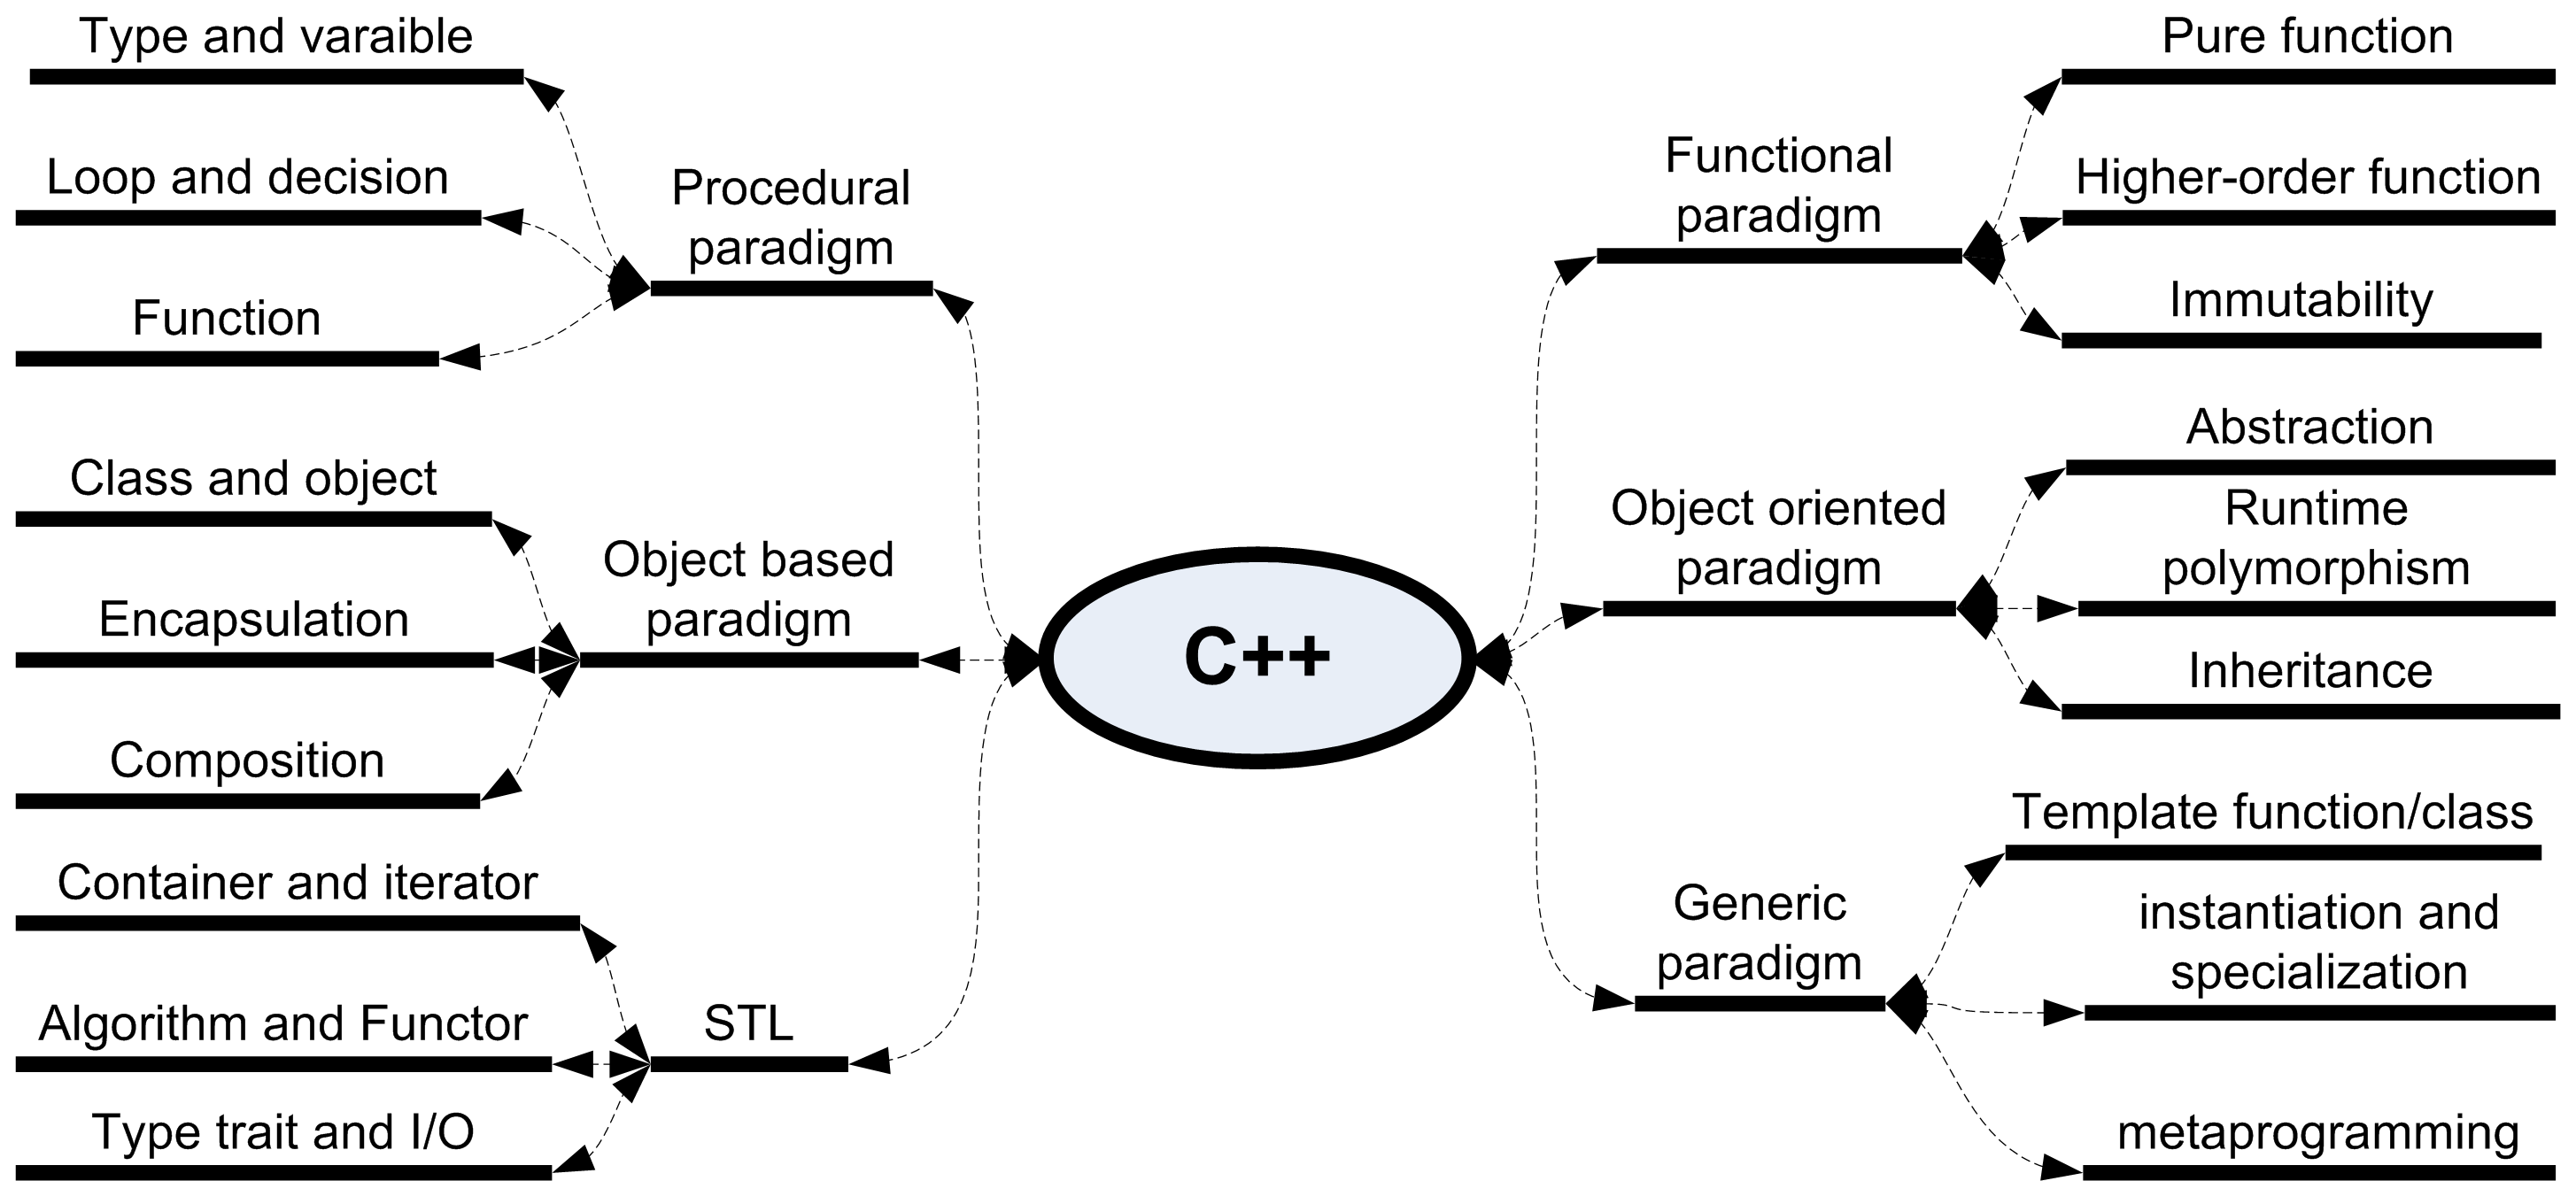
\includegraphics[width=0.85\linewidth]{pics/whole.png}
	%\caption{The main component of C++ language}
	
	
	
	\item C++ inherits basic data type, variable name, statement, expression, and operator, control flow, function, file, head file and library, array, pointer and structure from C language. C++ is superset of C, so any C programs can be compiled by C++.
	
	\item Duration and scope are two different conceptions in C++. there are three kinds of duration: \textbf{automatic, static and dynamic.} there are four kinds of scopes:
	\begin{enumerate}
		\item global.
		\item In C++, we can use namespace to add more scopes to divide global scope.
		\item file(translation unit).
		\item local, function local and class local. 
	\end{enumerate}
	
	\item Statement and expression are two important conceptions, you can see their definition in cppreference.com to see academic explanation.
	
	\item Statements are fragments of the C++ program that are executed in sequence. Only statement, which end with semicolon is executed. Most statements are expression statements. 
	\begin{lstlisting}
	int n = 1;               $\Hilight{3}$// declaration statement
	n = n + 1;               // expression statement
	std::cout << n << '\n'; // expression statement
	return 0;               // return statement stepnumber=1, 
	xleftmargin=1.2em, framexleftmargin=1.2em]
	int n = 1;               $\Hilight{3}$// declaration statement
	n = n + 1;               // expression statement
	std::cout << n << '\n'; // expression statement
	return 0;               // return statement
	stepnumber=1, xleftmargin=1.2em, framexleftmargin=1.2em]
	int n = 1;               $\Hilight{3}$// declaration statement
	n = n + 1;               // expression statement
	std::cout << n << '\n'; // expression statement
	return 0;               // return statement
	stepnumber=1, xleftmargin=1.2em, framexleftmargin=1.2em]
	int n = 1;               $\Hilight{3}$// declaration statement
	n = n + 1;               // expression statement
	std::cout << n << '\n'; // expression statement
	return 0;               // return statement
	\end{lstlisting}
	\begin{description}
		\item[line 1:] There is more than one word.An expression is a sequence of \textbf{operators} and their \textbf{operands}, that specifies a computation. Expression evaluation may produce a resultAn expression is a sequence of \textbf{operators} and their \textbf{operands}, that specifies a computation. Expression evaluation may produce a result
		\item[line 3:] An expression is a sequence of \textbf{operators} and their \textbf{operands}, that specifies a computation. Expression evaluation may produce a resultAn expression is a sequence of \textbf{operators} and their \textbf{operands}, that specifies a computation. Expression evaluation may produce a result
	\end{description}
	\begin{enumerate}
		\item An expression is a sequence of \textbf{operators} and their \textbf{operands}, that specifies a computation. Expression evaluation may produce a resultAn expression is a sequence of \textbf{operators} and their \textbf{operands}, that specifies a computation. Expression evaluation may produce a result
		
		\item An expression is a sequence of \textbf{operators} and their \textbf{operands}, that specifies a computation. Expression evaluation may produce a resultAn expression is a sequence of \textbf{operators} and their \textbf{operands}, that specifies a computation. Expression evaluation may produce a result
	\end{enumerate}
	\item An expression is a sequence of \textbf{operators} and their \textbf{operands}, that specifies a computation. Expression evaluation may produce a result
	
	\begin{enumerate}
		\item Expression: Something which evaluates to a value. Example: \texttt{1+2/x}
		\item Statement: A line of code which does something. Example: \texttt{GOTO 100;} and statements are all end with semi-comma.
	\end{enumerate}
	
	\item Function call is a expression, because it can yield a value.
	
	\item \textbf{All expressions yield a value, So expression is a value, statement is an action.}
	
	
	\item The designers of C realized that no harm was done if you were allowed to evaluate an expression and throw away the result. In C, every syntactic expression can be a made into a statement just by tacking a semicolon along the end:
	
	\begin{lstlisting}[numbers=none]
	x+y //is expression;
	x+y; //is statement, but you throw away the result
	j=i; is a statement.
	fun(i) //is expression;
	\end{lstlisting}
	
\end{itemize}


\subsection{basic definition}
\begin{itemize}
	
	\item gogo 
	
	
	\begin{tabular}{|c|c|c|}
		
		\textbf{type} & \textbf{read} & \textbf{write} \\
		
		primitive (char, int, float) & pass value & pointer or reference \\
		
		class, array, structure  & const pointer or reference &  pointer or reference  
	\end{tabular}
	\item gogo \newline
	
	
	
	\item gogo 
	
	\begin{tabular}{|p{0.3\textwidth}|p{0.3\textwidth}|p{0.3\textwidth}|}
		\tophline
		go go go go go go go let let let let let letgo go go go go go go let let let let let let &  go go go go go go go let let let let let letgo go go go go go go let let let let let let&
		go go go go go go go let let let let let letgo go go go go go go let let let let let let  
		\\ \tophline
		
		primitive (char, int, float) & pass value & pointer or reference \\ \tophline
		class, array, structure  & const pointer or reference &  pointer or reference \bottomhline
	\end{tabular}
	
	
	\item C++ is a Multi-paradigm language, there are five paradigms: 
	
	\begin{enumerate}
		\item Procedural programming. (traditional C programming)
		\item Object-base programming. (class and object)
		\item Object-orient programming. (inheritance)
		\item Generic programming. (template)
		\item functional programming
	\end{enumerate}
	
	
	%\centering
	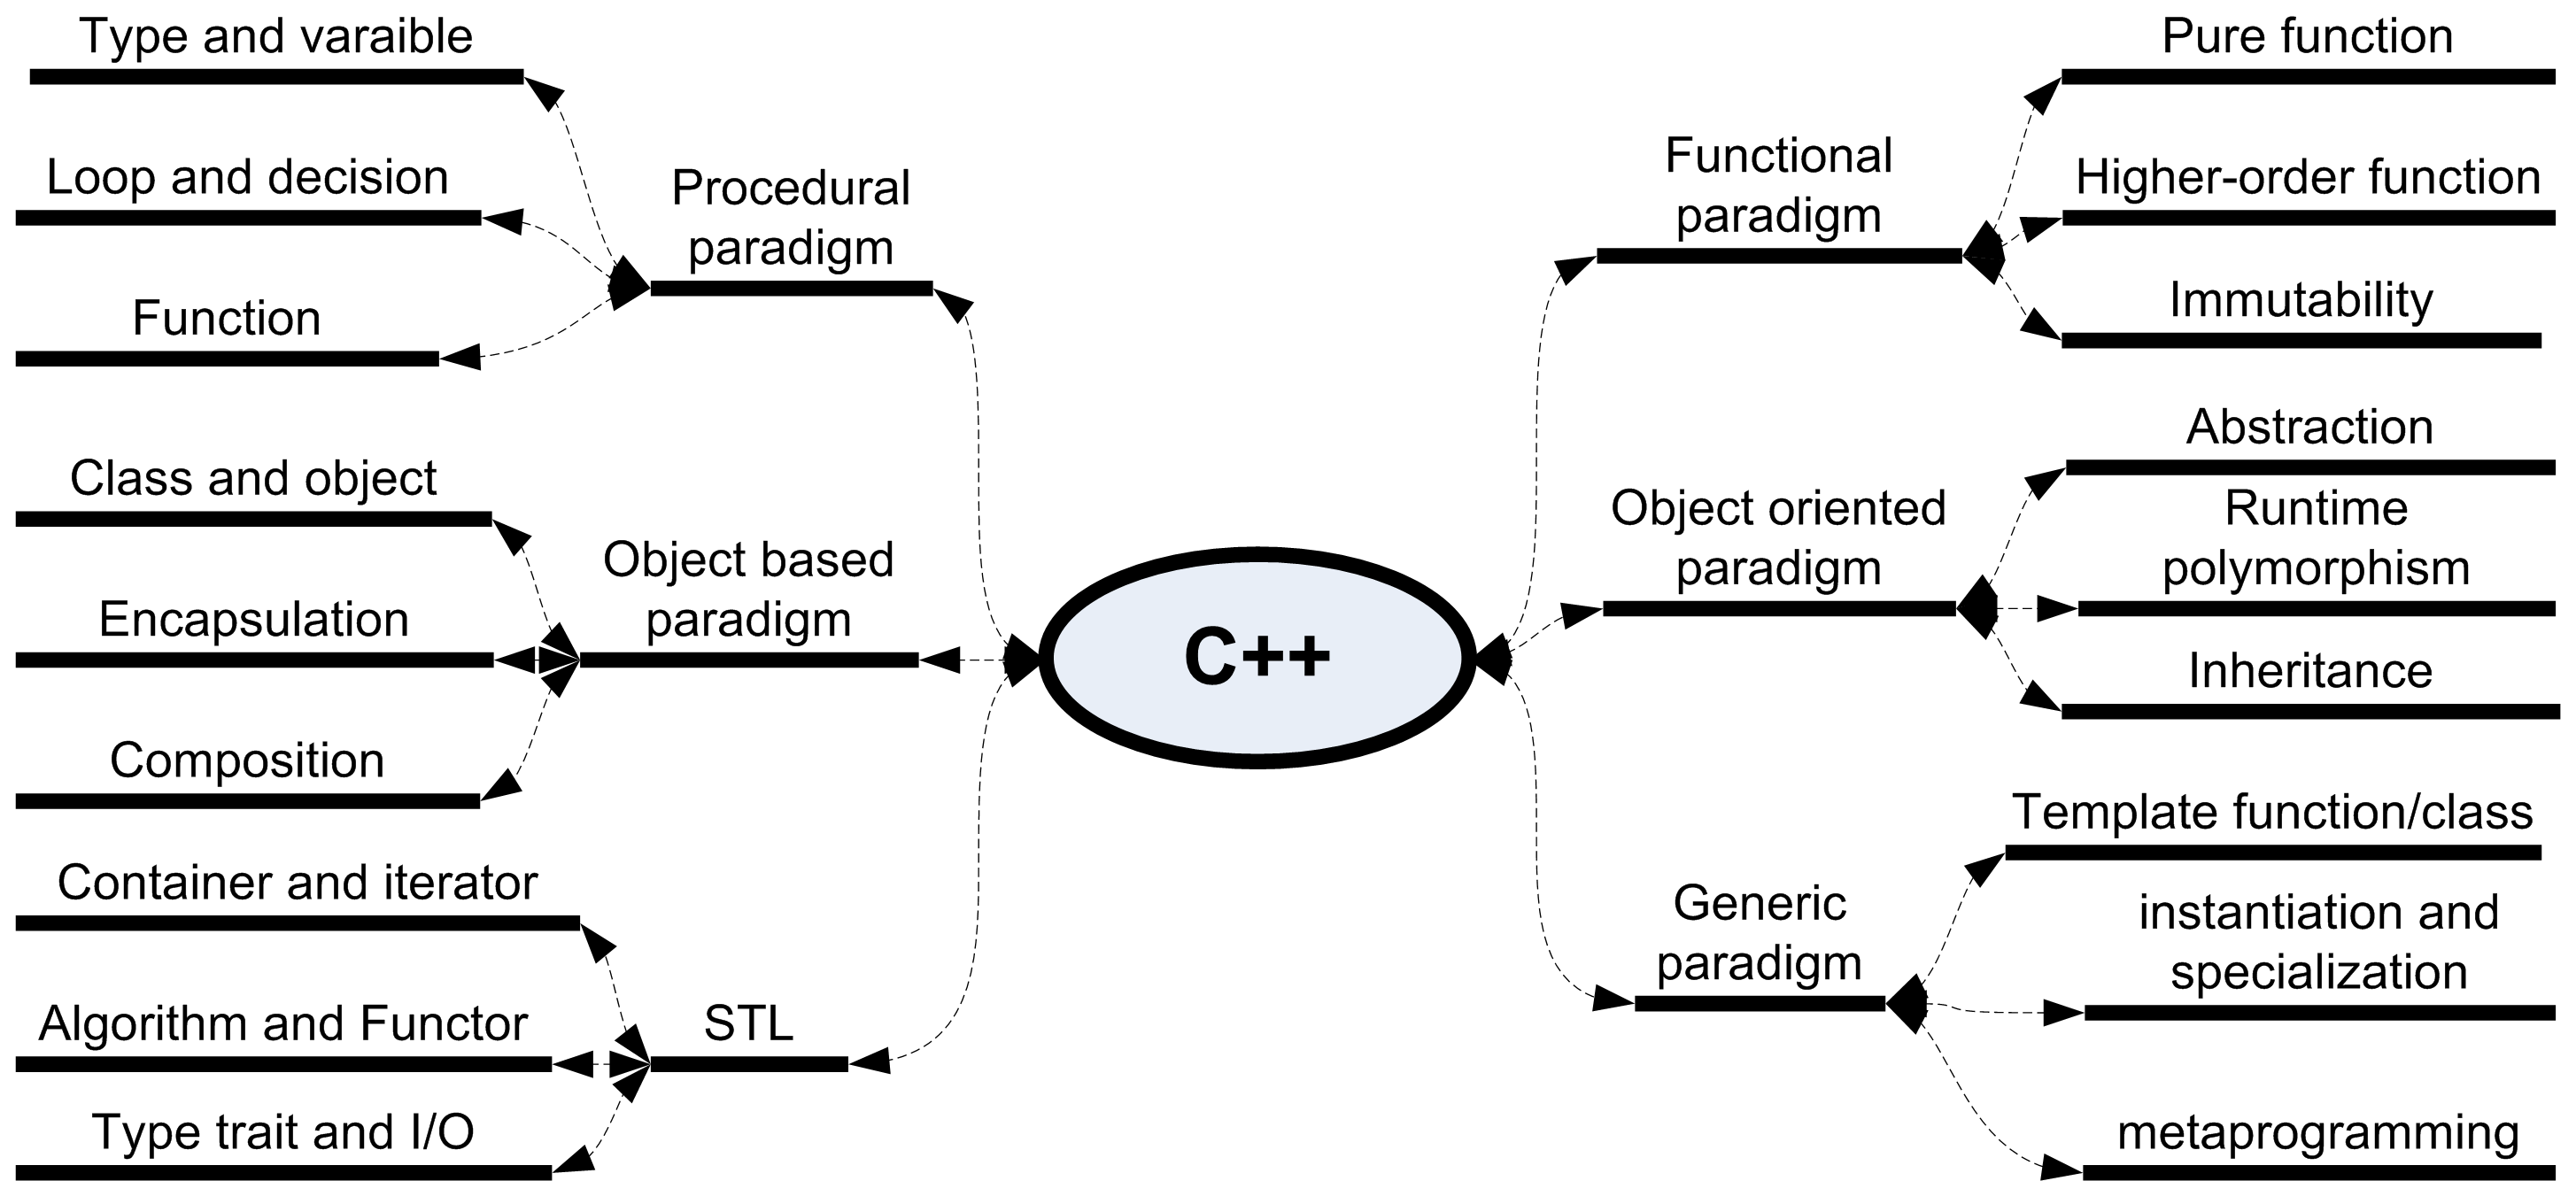
\includegraphics[width=0.85\linewidth]{pics/whole.png}
	%\caption{The main component of C++ language}
	
	
	
	\item C++ inherits basic data type, variable name, statement, expression, and operator, control flow, function, file, head file and library, array, pointer and structure from C language. C++ is superset of C, so any C programs can be compiled by C++.
	
	\item Duration and scope are two different conceptions in C++. there are three kinds of duration: \textbf{automatic, static and dynamic.} there are four kinds of scopes:
	\begin{enumerate}
		\item global.
		\item In C++, we can use namespace to add more scopes to divide global scope.
		\item file(translation unit).
		\item local, function local and class local. 
	\end{enumerate}
	
	\item Statement and expression are two important conceptions, you can see their definition in cppreference.com to see academic explanation.
	
	\item Statements are fragments of the C++ program that are executed in sequence. Only statement, which end with semicolon is executed. Most statements are expression statements. 
	\begin{lstlisting}
	int n = 1;               $\Hilight{3}$// declaration statement
	n = n + 1;               // expression statement
	std::cout << n << '\n'; // expression statement
	return 0;               // return statement stepnumber=1, 
	xleftmargin=1.2em, framexleftmargin=1.2em]
	int n = 1;               $\Hilight{3}$// declaration statement
	n = n + 1;               // expression statement
	std::cout << n << '\n'; // expression statement
	return 0;               // return statement
	stepnumber=1, xleftmargin=1.2em, framexleftmargin=1.2em]
	int n = 1;               $\Hilight{3}$// declaration statement
	n = n + 1;               // expression statement
	std::cout << n << '\n'; // expression statement
	return 0;               // return statement
	stepnumber=1, xleftmargin=1.2em, framexleftmargin=1.2em]
	int n = 1;               $\Hilight{3}$// declaration statement
	n = n + 1;               // expression statement
	std::cout << n << '\n'; // expression statement
	return 0;               // return statement
	\end{lstlisting}
	\begin{description}
		\item[line 1:] There is more than one word.An expression is a sequence of \textbf{operators} and their \textbf{operands}, that specifies a computation. Expression evaluation may produce a resultAn expression is a sequence of \textbf{operators} and their \textbf{operands}, that specifies a computation. Expression evaluation may produce a result
		\item[line 3:] An expression is a sequence of \textbf{operators} and their \textbf{operands}, that specifies a computation. Expression evaluation may produce a resultAn expression is a sequence of \textbf{operators} and their \textbf{operands}, that specifies a computation. Expression evaluation may produce a result
	\end{description}
	\begin{enumerate}
		\item An expression is a sequence of \textbf{operators} and their \textbf{operands}, that specifies a computation. Expression evaluation may produce a resultAn expression is a sequence of \textbf{operators} and their \textbf{operands}, that specifies a computation. Expression evaluation may produce a result
		
		\item An expression is a sequence of \textbf{operators} and their \textbf{operands}, that specifies a computation. Expression evaluation may produce a resultAn expression is a sequence of \textbf{operators} and their \textbf{operands}, that specifies a computation. Expression evaluation may produce a result
	\end{enumerate}
	\item An expression is a sequence of \textbf{operators} and their \textbf{operands}, that specifies a computation. Expression evaluation may produce a result
	
	\begin{enumerate}
		\item Expression: Something which evaluates to a value. Example: \texttt{1+2/x}
		\item Statement: A line of code which does something. Example: \texttt{GOTO 100;} and statements are all end with semi-comma.
	\end{enumerate}
	
	\item Function call is a expression, because it can yield a value.
	
	\item \textbf{All expressions yield a value, So expression is a value, statement is an action.}
	
	
	\item The designers of C realized that no harm was done if you were allowed to evaluate an expression and throw away the result. In C, every syntactic expression can be a made into a statement just by tacking a semicolon along the end:
	
	\begin{lstlisting}[numbers=none]
	x+y //is expression;
	x+y; //is statement, but you throw away the result
	j=i; is a statement.
	fun(i) //is expression;
	\end{lstlisting}
	
\end{itemize}


\subsection{basic definition}
\begin{itemize}
	
	\item gogo 
	
	
	\begin{tabular}{|c|c|c|}
		
		\textbf{type} & \textbf{read} & \textbf{write} \\
		
		primitive (char, int, float) & pass value & pointer or reference \\
		
		class, array, structure  & const pointer or reference &  pointer or reference  
	\end{tabular}
	\item gogo \newline
	
	
	
	\item gogo 
	
	\begin{tabular}{|p{0.3\textwidth}|p{0.3\textwidth}|p{0.3\textwidth}|}
		\tophline
		go go go go go go go let let let let let letgo go go go go go go let let let let let let &  go go go go go go go let let let let let letgo go go go go go go let let let let let let&
		go go go go go go go let let let let let letgo go go go go go go let let let let let let  
		\\ \tophline
		
		primitive (char, int, float) & pass value & pointer or reference \\ \tophline
		class, array, structure  & const pointer or reference &  pointer or reference \bottomhline
	\end{tabular}
	
	
	\item C++ is a Multi-paradigm language, there are five paradigms: 
	
	\begin{enumerate}
		\item Procedural programming. (traditional C programming)
		\item Object-base programming. (class and object)
		\item Object-orient programming. (inheritance)
		\item Generic programming. (template)
		\item functional programming
	\end{enumerate}
	
	
	%\centering
	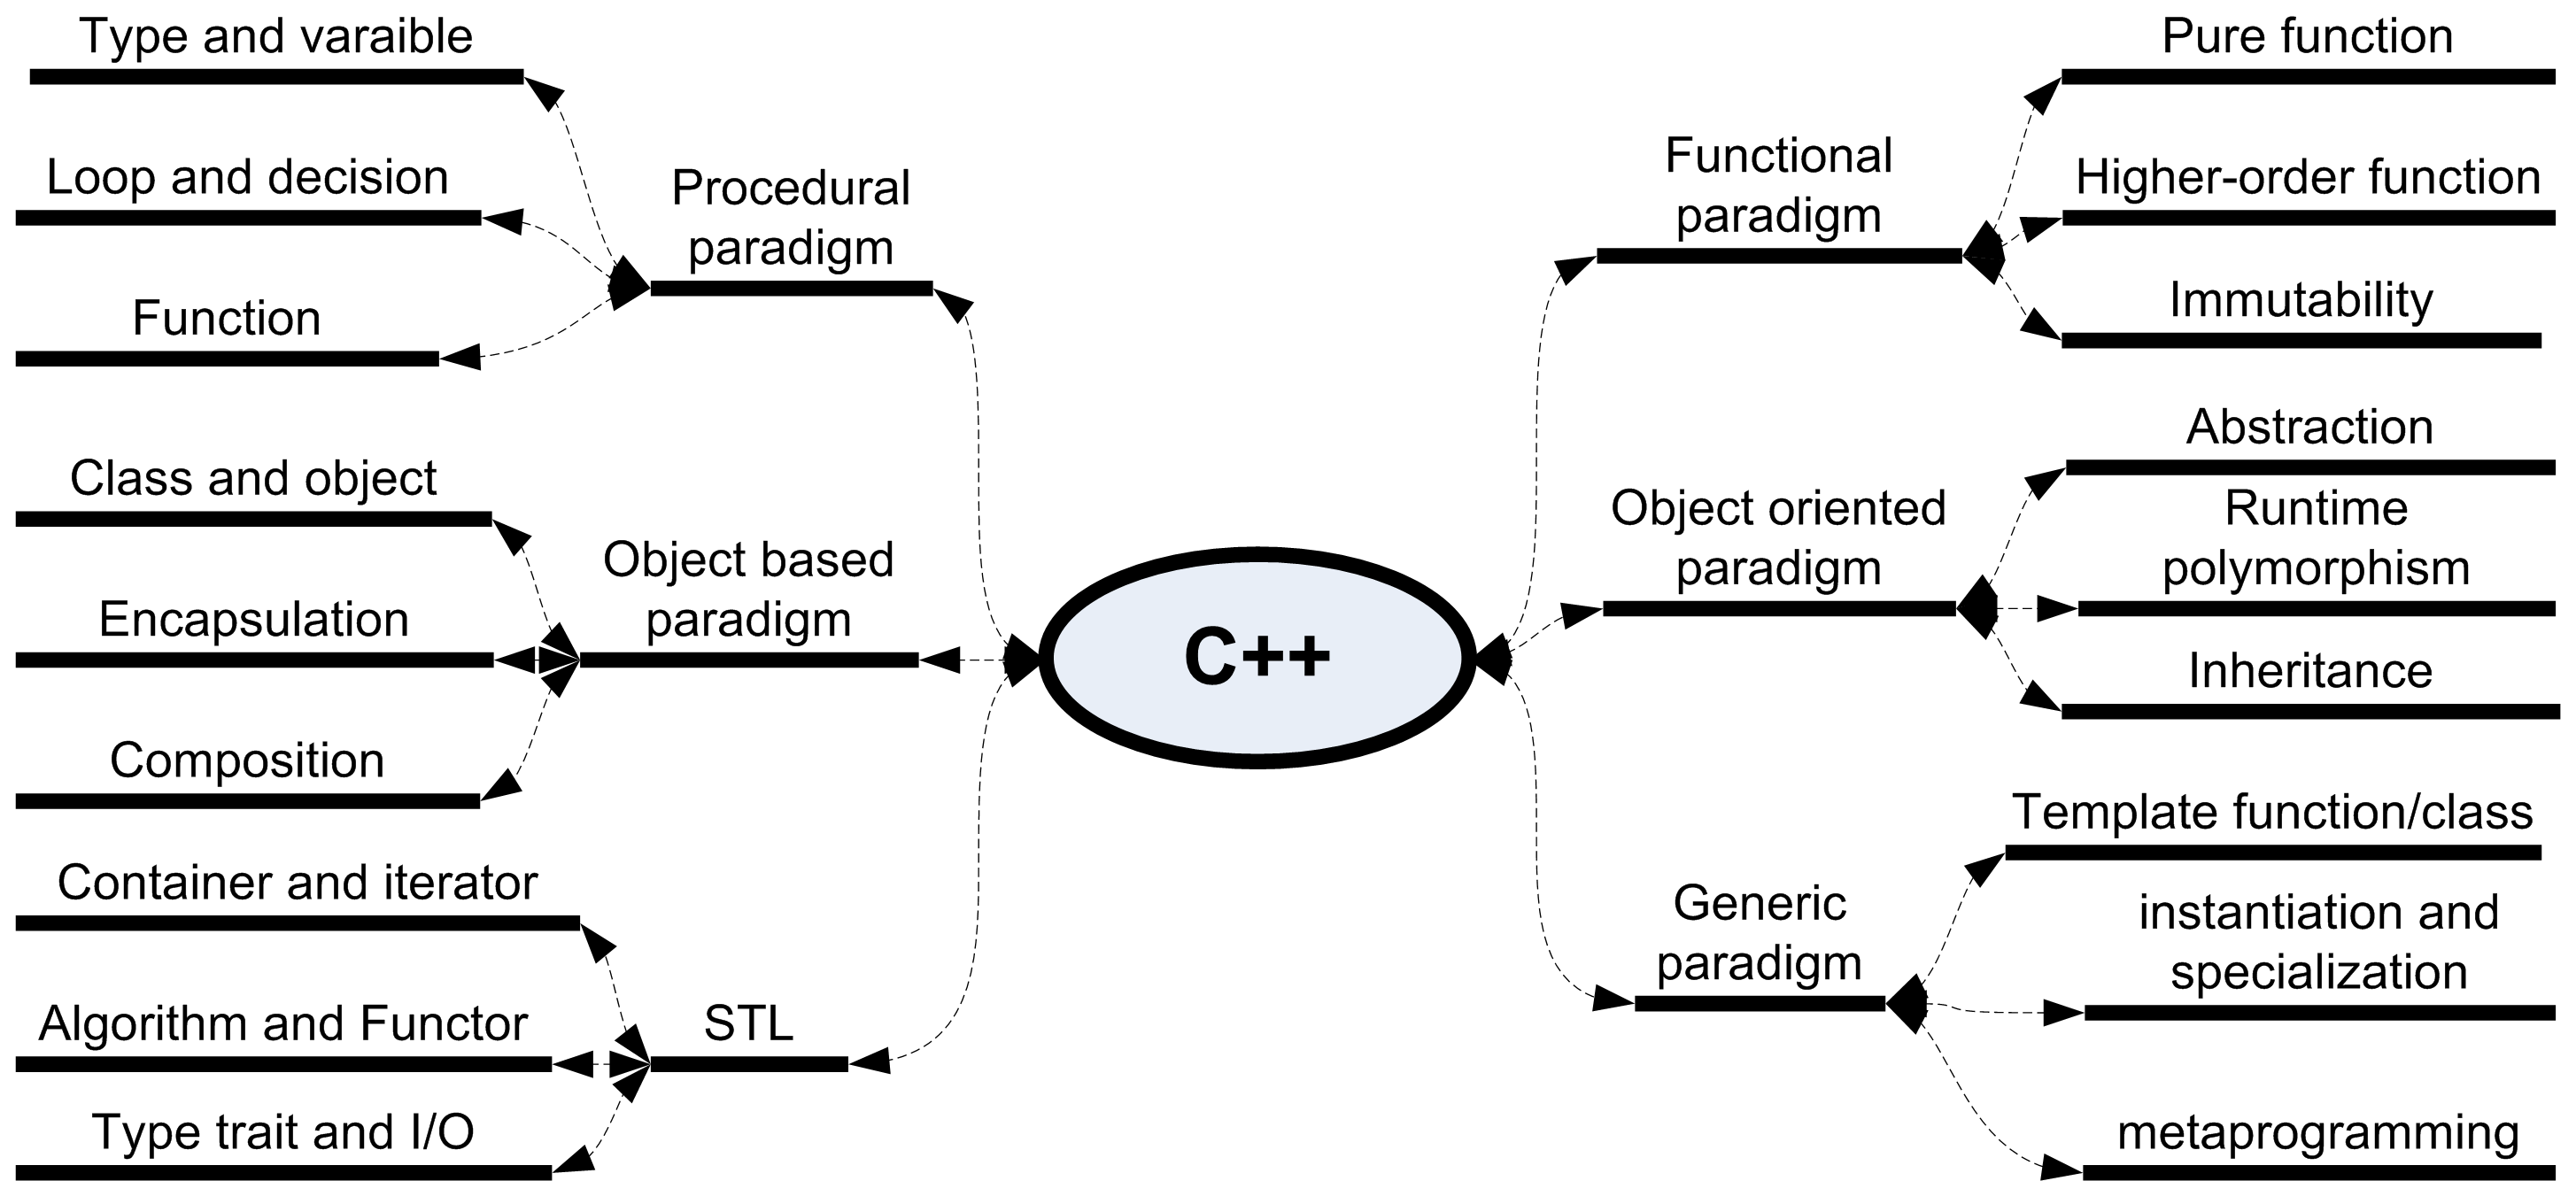
\includegraphics[width=0.85\linewidth]{pics/whole.png}
	%\caption{The main component of C++ language}
	
	
	
	\item C++ inherits basic data type, variable name, statement, expression, and operator, control flow, function, file, head file and library, array, pointer and structure from C language. C++ is superset of C, so any C programs can be compiled by C++.
	
	\item Duration and scope are two different conceptions in C++. there are three kinds of duration: \textbf{automatic, static and dynamic.} there are four kinds of scopes:
	\begin{enumerate}
		\item global.
		\item In C++, we can use namespace to add more scopes to divide global scope.
		\item file(translation unit).
		\item local, function local and class local. 
	\end{enumerate}
	
	\item Statement and expression are two important conceptions, you can see their definition in cppreference.com to see academic explanation.
	
	\item Statements are fragments of the C++ program that are executed in sequence. Only statement, which end with semicolon is executed. Most statements are expression statements. 
	\begin{lstlisting}
	int n = 1;               $\Hilight{3}$// declaration statement
	n = n + 1;               // expression statement
	std::cout << n << '\n'; // expression statement
	return 0;               // return statement stepnumber=1, 
	xleftmargin=1.2em, framexleftmargin=1.2em]
	int n = 1;               $\Hilight{3}$// declaration statement
	n = n + 1;               // expression statement
	std::cout << n << '\n'; // expression statement
	return 0;               // return statement
	stepnumber=1, xleftmargin=1.2em, framexleftmargin=1.2em]
	int n = 1;               $\Hilight{3}$// declaration statement
	n = n + 1;               // expression statement
	std::cout << n << '\n'; // expression statement
	return 0;               // return statement
	stepnumber=1, xleftmargin=1.2em, framexleftmargin=1.2em]
	int n = 1;               $\Hilight{3}$// declaration statement
	n = n + 1;               // expression statement
	std::cout << n << '\n'; // expression statement
	return 0;               // return statement
	\end{lstlisting}
	\begin{description}
		\item[line 1:] There is more than one word.An expression is a sequence of \textbf{operators} and their \textbf{operands}, that specifies a computation. Expression evaluation may produce a resultAn expression is a sequence of \textbf{operators} and their \textbf{operands}, that specifies a computation. Expression evaluation may produce a result
		\item[line 3:] An expression is a sequence of \textbf{operators} and their \textbf{operands}, that specifies a computation. Expression evaluation may produce a resultAn expression is a sequence of \textbf{operators} and their \textbf{operands}, that specifies a computation. Expression evaluation may produce a result
	\end{description}
	\begin{enumerate}
		\item An expression is a sequence of \textbf{operators} and their \textbf{operands}, that specifies a computation. Expression evaluation may produce a resultAn expression is a sequence of \textbf{operators} and their \textbf{operands}, that specifies a computation. Expression evaluation may produce a result
		
		\item An expression is a sequence of \textbf{operators} and their \textbf{operands}, that specifies a computation. Expression evaluation may produce a resultAn expression is a sequence of \textbf{operators} and their \textbf{operands}, that specifies a computation. Expression evaluation may produce a result
	\end{enumerate}
	\item An expression is a sequence of \textbf{operators} and their \textbf{operands}, that specifies a computation. Expression evaluation may produce a result
	
	\begin{enumerate}
		\item Expression: Something which evaluates to a value. Example: \texttt{1+2/x}
		\item Statement: A line of code which does something. Example: \texttt{GOTO 100;} and statements are all end with semi-comma.
	\end{enumerate}
	
	\item Function call is a expression, because it can yield a value.
	
	\item \textbf{All expressions yield a value, So expression is a value, statement is an action.}
	
	
	\item The designers of C realized that no harm was done if you were allowed to evaluate an expression and throw away the result. In C, every syntactic expression can be a made into a statement just by tacking a semicolon along the end:
	
	\begin{lstlisting}[numbers=none]
	x+y //is expression;
	x+y; //is statement, but you throw away the result
	j=i; is a statement.
	fun(i) //is expression;
	\end{lstlisting}
	
\end{itemize}

\subsection{basic definition}
\begin{itemize}
	
	\item gogo 
	
	
	\begin{tabular}{|c|c|c|}
		
		\textbf{type} & \textbf{read} & \textbf{write} \\
		
		primitive (char, int, float) & pass value & pointer or reference \\
		
		class, array, structure  & const pointer or reference &  pointer or reference  
	\end{tabular}
	\item gogo \newline
	
	
	
	\item gogo 
	
	\begin{tabular}{|p{0.3\textwidth}|p{0.3\textwidth}|p{0.3\textwidth}|}
		\tophline
		go go go go go go go let let let let let letgo go go go go go go let let let let let let &  go go go go go go go let let let let let letgo go go go go go go let let let let let let&
		go go go go go go go let let let let let letgo go go go go go go let let let let let let  
		\\ \tophline
		
		primitive (char, int, float) & pass value & pointer or reference \\ \tophline
		class, array, structure  & const pointer or reference &  pointer or reference \bottomhline
	\end{tabular}
	
	
	\item C++ is a Multi-paradigm language, there are five paradigms: 
	
	\begin{enumerate}
		\item Procedural programming. (traditional C programming)
		\item Object-base programming. (class and object)
		\item Object-orient programming. (inheritance)
		\item Generic programming. (template)
		\item functional programming
	\end{enumerate}
	
	
	%\centering
	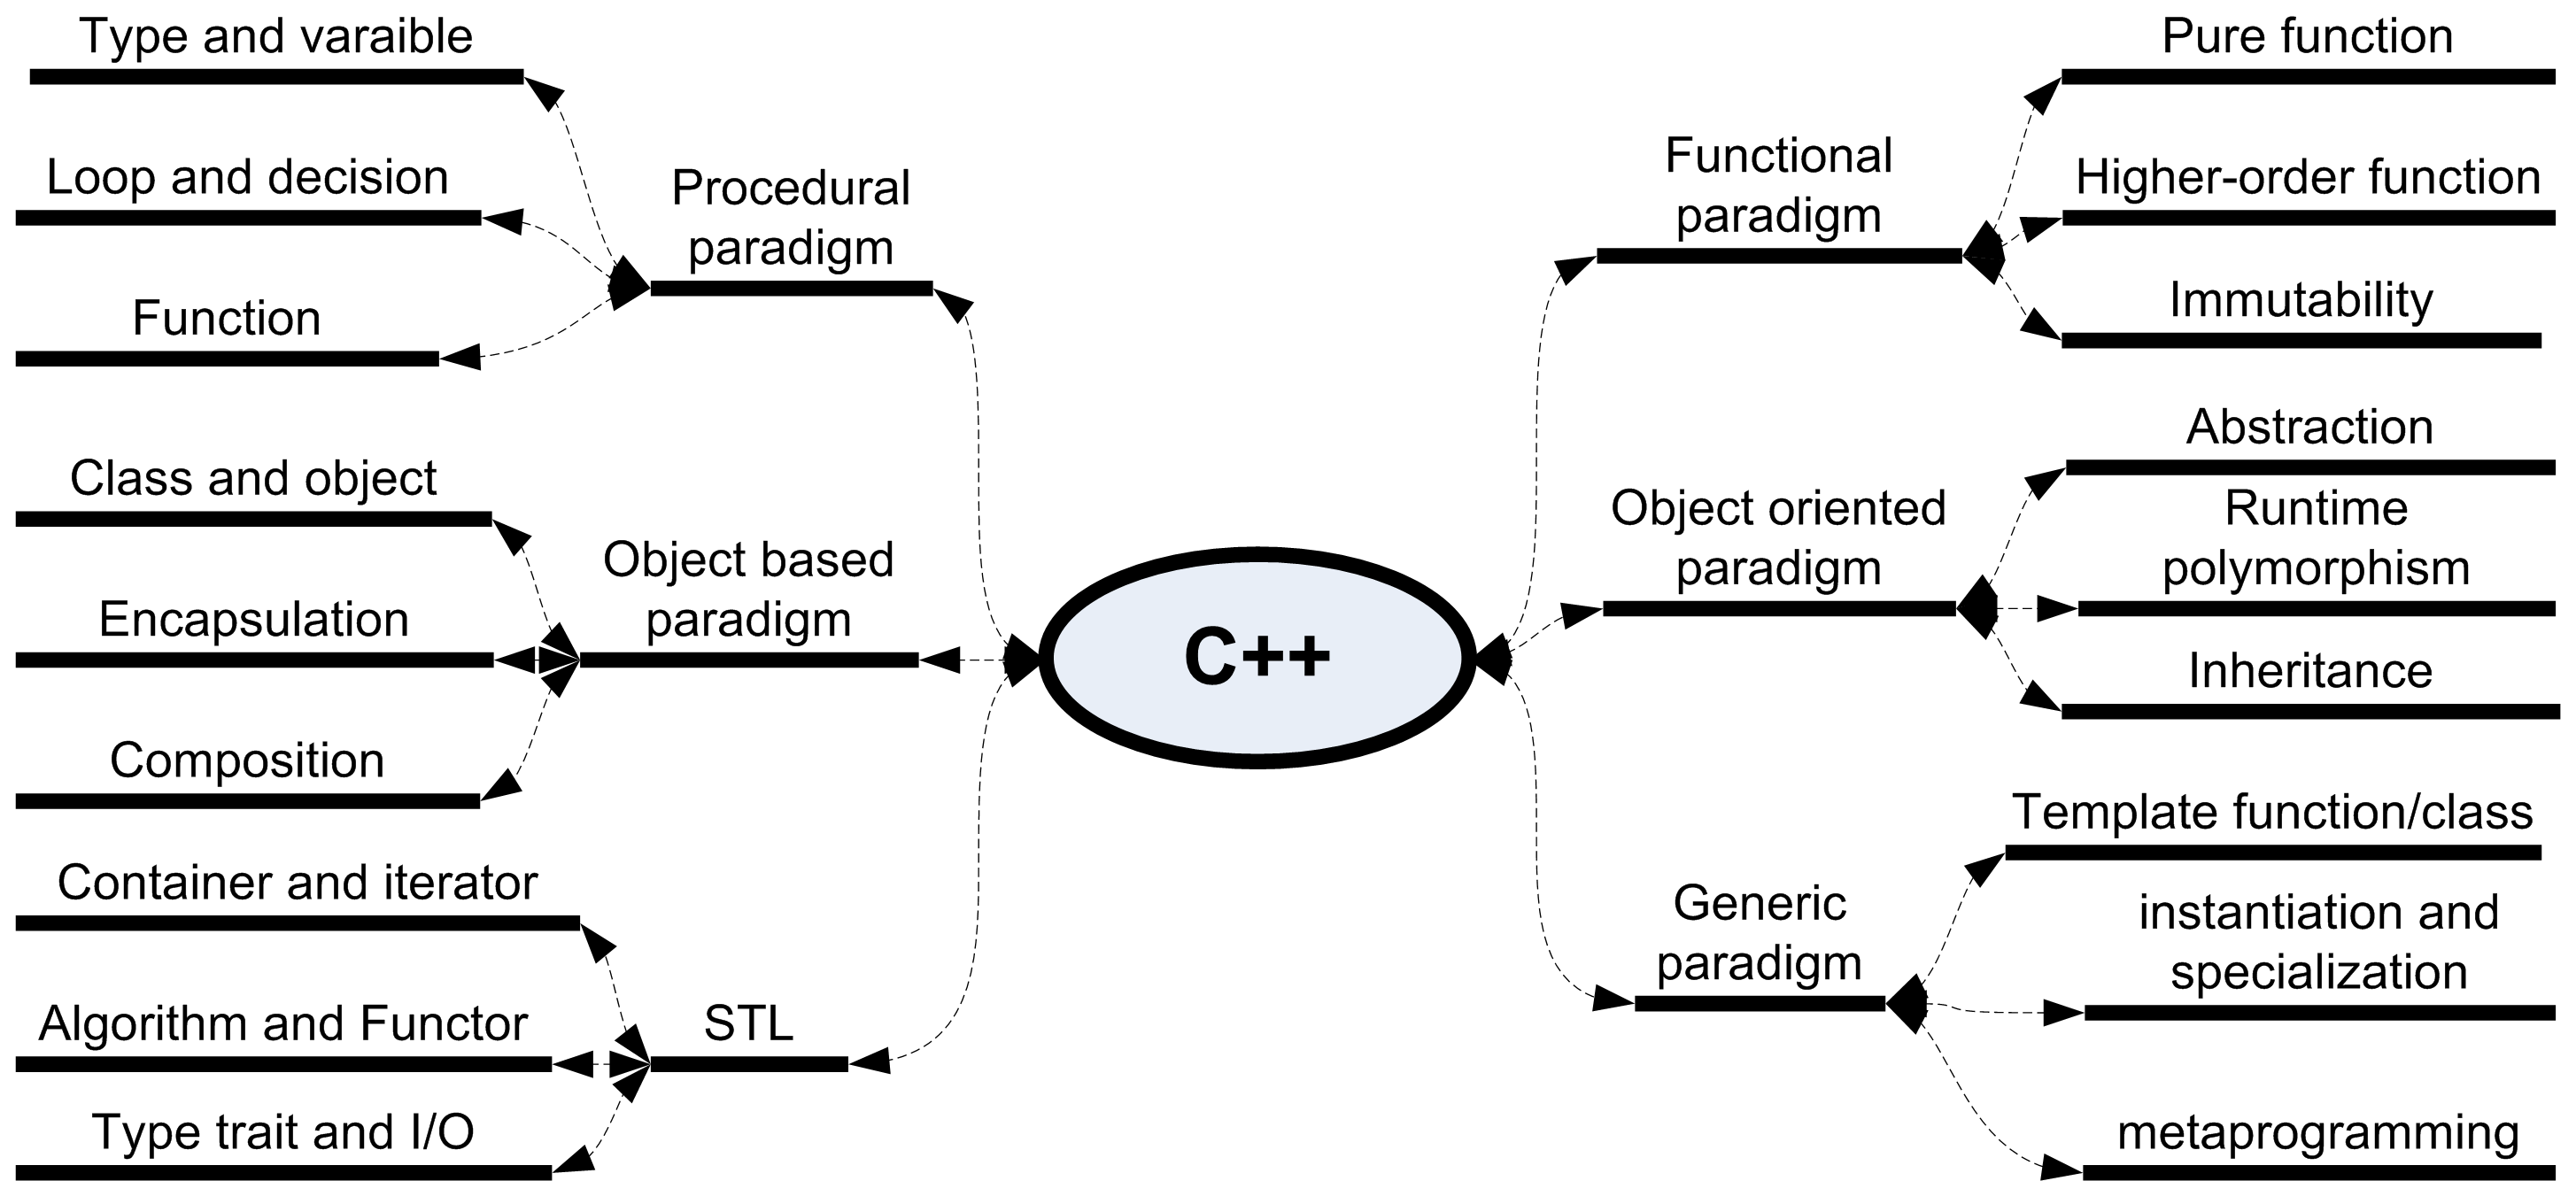
\includegraphics[width=0.85\linewidth]{pics/whole.png}
	%\caption{The main component of C++ language}
	
	
	
	\item C++ inherits basic data type, variable name, statement, expression, and operator, control flow, function, file, head file and library, array, pointer and structure from C language. C++ is superset of C, so any C programs can be compiled by C++.
	
	\item Duration and scope are two different conceptions in C++. there are three kinds of duration: \textbf{automatic, static and dynamic.} there are four kinds of scopes:
	\begin{enumerate}
		\item global.
		\item In C++, we can use namespace to add more scopes to divide global scope.
		\item file(translation unit).
		\item local, function local and class local. 
	\end{enumerate}
	
	\item Statement and expression are two important conceptions, you can see their definition in cppreference.com to see academic explanation.
	
	\item Statements are fragments of the C++ program that are executed in sequence. Only statement, which end with semicolon is executed. Most statements are expression statements. 
	\begin{lstlisting}
	int n = 1;               $\Hilight{3}$// declaration statement
	n = n + 1;               // expression statement
	std::cout << n << '\n'; // expression statement
	return 0;               // return statement stepnumber=1, 
	xleftmargin=1.2em, framexleftmargin=1.2em]
	int n = 1;               $\Hilight{3}$// declaration statement
	n = n + 1;               // expression statement
	std::cout << n << '\n'; // expression statement
	return 0;               // return statement
	stepnumber=1, xleftmargin=1.2em, framexleftmargin=1.2em]
	int n = 1;               $\Hilight{3}$// declaration statement
	n = n + 1;               // expression statement
	std::cout << n << '\n'; // expression statement
	return 0;               // return statement
	stepnumber=1, xleftmargin=1.2em, framexleftmargin=1.2em]
	int n = 1;               $\Hilight{3}$// declaration statement
	n = n + 1;               // expression statement
	std::cout << n << '\n'; // expression statement
	return 0;               // return statement
	\end{lstlisting}
	\begin{description}
		\item[line 1:] There is more than one word.An expression is a sequence of \textbf{operators} and their \textbf{operands}, that specifies a computation. Expression evaluation may produce a resultAn expression is a sequence of \textbf{operators} and their \textbf{operands}, that specifies a computation. Expression evaluation may produce a result
		\item[line 3:] An expression is a sequence of \textbf{operators} and their \textbf{operands}, that specifies a computation. Expression evaluation may produce a resultAn expression is a sequence of \textbf{operators} and their \textbf{operands}, that specifies a computation. Expression evaluation may produce a result
	\end{description}
	\begin{enumerate}
		\item An expression is a sequence of \textbf{operators} and their \textbf{operands}, that specifies a computation. Expression evaluation may produce a resultAn expression is a sequence of \textbf{operators} and their \textbf{operands}, that specifies a computation. Expression evaluation may produce a result
		
		\item An expression is a sequence of \textbf{operators} and their \textbf{operands}, that specifies a computation. Expression evaluation may produce a resultAn expression is a sequence of \textbf{operators} and their \textbf{operands}, that specifies a computation. Expression evaluation may produce a result
	\end{enumerate}
	\item An expression is a sequence of \textbf{operators} and their \textbf{operands}, that specifies a computation. Expression evaluation may produce a result
	
	\begin{enumerate}
		\item Expression: Something which evaluates to a value. Example: \texttt{1+2/x}
		\item Statement: A line of code which does something. Example: \texttt{GOTO 100;} and statements are all end with semi-comma.
	\end{enumerate}
	
	\item Function call is a expression, because it can yield a value.
	
	\item \textbf{All expressions yield a value, So expression is a value, statement is an action.}
	
	
	\item The designers of C realized that no harm was done if you were allowed to evaluate an expression and throw away the result. In C, every syntactic expression can be a made into a statement just by tacking a semicolon along the end:
	
	\begin{lstlisting}[numbers=none]
	x+y //is expression;
	x+y; //is statement, but you throw away the result
	j=i; is a statement.
	fun(i) //is expression;
	\end{lstlisting}
	
\end{itemize}





\end{document}

